\chapter{Indexation par termes-clés\index{terme-cle@Terme-clé} en domaines\index{domaine@Domaine} de spécialité\index{specialite@Spécialité}}
\label{chap:main-domain_specific_keyphrase_annotation}
  \chaptercite{
    La multiplication des bases de données et l'information devenue
    \og{}marché\fg{} (donc rentable) ont entraîné d'autres corps de métier à
    s'intéresser à la pratique de l'indexation. Mais ce sont les bibliothécaires
    et documentalistes qui en ont défini les méthodes\index{methode@Méthode}, les usages et les outils.
  }{
    \newcite{guinchat1996techniquesdocumentaires}
  }{.75\linewidth}{\justify}

  %-----------------------------------------------------------------------------

  \section{Introduction}
  \label{sec:main:domain_specific_keyphrase_annotation-introduction}
    Dans ce chapitre, nous nous intéressons à l'indexation par
    termes-clés\index{terme-cle@Terme-clé} en domaines\index{domaine@Domaine} de spécialité\index{specialite@Spécialité}. Dans la littérature, l'indexation
    par termes-clés\index{terme-cle@Terme-clé} se divise en deux catégories~: l'extraction de termes-clés\index{terme-cle@Terme-clé},
    qui fournit des termes-clés\index{terme-cle@Terme-clé} apparaissant dans le contenu du document\index{document@Document}, et
    l'assignement de termes-clés\index{terme-cle@Terme-clé}, qui fournit des termes-clés\index{terme-cle@Terme-clé} appartenant à un
    vocabulaire\index{vocabulaire@Vocabulaire} contrôlé et n'apparaissant pas nécessairement dans le document\index{document@Document}.
    Alors que dans la littérature, l'indexation par termes-clés\index{terme-cle@Terme-clé} est
    principalement réalisée au seul moyen de l'extraction de termes-clés\index{terme-cle@Terme-clé}, nous
    montrons que l'assignement de termes-clés\index{terme-cle@Terme-clé} joue un rôle important en domaines\index{domaine@Domaine}
    de spécialité\index{specialite@Spécialité}.

    Nous commençons par décrire le comportement des indexeurs
    professionnels qui maintiennent les bases des données bibliographiques de
    l'Inist (Institut de l'information scientifique et technique), puis nous en
    proposons une automatisation. Les indexeurs professionnels assignent à
    chaque document\index{document@Document} des termes-clés\index{terme-cle@Terme-clé} du domaine\index{domaine@Domaine} (d'un vocabulaire\index{vocabulaire@Vocabulaire} contrôlé), et
    extraient des termes-clés\index{terme-cle@Terme-clé} spécifiques au document\index{document@Document} (hors du vocabulaire\index{vocabulaire@Vocabulaire}
    contrôlé), voir des concepts nouveaux dans le domaine\index{domaine@Domaine}. Pour reproduire ce comportement, nous étendons nos travaux sur
    TopicRank\index{topicrank@TopicRank} en intégrant dans le graphe\index{graphe@Graphe} de sujets\index{sujet@Sujet} les entrées du vocabulaire\index{vocabulaire@Vocabulaire}
    du domaine\index{domaine@Domaine}.

    Enfin, nous présentons les premiers résultats\index{resultat@Résultat} d'une campagne d'évaluation
    manuelle de nos travaux en domaines\index{domaine@Domaine} de spécialité\index{specialite@Spécialité}. Pour cette campagne,
    nous proposons un protocole et des métriques permettant d'évaluer deux
    aspects~: la pertinence des termes-clés\index{terme-cle@Terme-clé} extraits/assignés et la quantité
    d'information importante capturée par les termes-clés\index{terme-cle@Terme-clé}.

  %-----------------------------------------------------------------------------

  \section{Indexation manuelle en domaines\index{domaine@Domaine} de spécialité\index{specialite@Spécialité}}
  \label{sec:main-domain_specific_keyphrase_annotation-manual_keyphrase_annotation}
    En nous fondant sur les  propos recueillis auprès des indexeurs
    professionnels de l'Inist, qui maintient une partie des bases de données
    bibliographiques de la \textsc{Bsn} (Bibliothèque scientifique numérique),
    nous présentons la méthodologie d'indexation manuelle en domaines\index{domaine@Domaine} de
    spécialité\index{specialite@Spécialité}.

    \subsection{Principes généraux}
    \label{subsec:main-domain_specific_keyphrase_annotation-manual_keyphrase_annotation-principles}
      L'indexation manuelle de l'Inist est régie par cinq principes généraux~:
      \begin{enumerate}
        \item{Conformité~: les termes-clés\index{terme-cle@Terme-clé} doivent être conformes au contenu du
              document\index{document@Document} et au langage documentaire utilisé dans son domaine\index{domaine@Domaine}~;}
        \item{Exhaustivité~: les termes-clés\index{terme-cle@Terme-clé} doivent représenter tous les
              aspects importants du document\index{document@Document}, même lorsque ceux-ci sont
              implicites~;}
        \item{Homogénéité~: les termes-clés\index{terme-cle@Terme-clé} des documents\index{document@Document} d'un même domaine\index{domaine@Domaine}
              doivent être cohérents et identiques lorsqu'ils représentent le
              même concept~;}
        \item{Spécificité~: les termes-clés\index{terme-cle@Terme-clé} doivent décrire le contenu d'un
              document\index{document@Document} au niveau le plus spécifique et peuvent
              parfois être accompagnés de termes-clés\index{terme-cle@Terme-clé} plus génériques afin de
              restituer le contenu du document\index{document@Document} dans son domaine\index{domaine@Domaine}~;}
        \item{Impartialité~: les termes-clés\index{terme-cle@Terme-clé} ne doivent pas être représentatifs
              d'un jugement apporté par l'indexeur.}
      \end{enumerate}

      Ces principes généraux de l'indexation manuelle par termes-clés\index{terme-cle@Terme-clé} remettent
      en cause la séparation entre extraction et assignement de termes-clés\index{terme-cle@Terme-clé} dans
      le contexte de l'indexation automatique\index{indexation automatique@Indexation automatique} en domaines\index{domaine@Domaine} de spécialité\index{specialite@Spécialité}. En
      effet, une indexation par termes-clés\index{terme-cle@Terme-clé} à un niveau professionnel doit
      respecter le langage de spécialité\index{specialite@Spécialité} employé dans le domaine\index{domaine@Domaine} des documents\index{document@Document}
      indexés (tâche d'assignement), mais elle doit aussi être exhaustive et
      donc fournir des termes-clés\index{terme-cle@Terme-clé} très spécifiques, voir de nouveaux concepts
      (tâche d'extraction).

    \subsection{Ressources}
    \label{subsec:main-domain_specific_keyphrase_annotation-manual_keyphrase_annotation-resources}
      L'indexation par termes-clés\index{terme-cle@Terme-clé} réalisée par les indexeurs professionnels de
      l'Inist s'appuie sur plusieurs ressources. Ces dernières sont
      représentatives d'une expertise de terrain dans chaque domaine\index{domaine@Domaine} de
      spécialité\index{specialite@Spécialité} (grille d'indexation), d'une expertise terminologique
      (vocabulaire\index{vocabulaire@Vocabulaire} contrôlé) et d'une expertise documentaire (règles de
      préindexation). Elles assurent des conditions de travail propices
      au respect des cinq principes généraux énoncés précédemment.

      \subsubsection{Grille d'indexation}
      \label{subsubsec:main-domain_specific_keyphrase_annotation-manual_keyphrase_annotation-resources-indexing_guidelines}
        De nos jours, la grille d'indexation est un guide transmis de manière
        informelle aux indexeurs. Elle indique les notions à indexer selon le
        domaine\index{domaine@Domaine} de spécialité\index{specialite@Spécialité} et peut se traduire par un formulaire à compléter
        pour chaque document\index{document@Document} (voir le tableau\index{tableau@Tableau}~\ref{fig:indexing_grid}). C'est un
        canevas donné à titre indicatif aux indexeurs. Ces derniers sont les
        seuls juges pour décider si elle est adaptée ou non pour indexer un
        document\index{document@Document}.
        \begin{table}[h!]
          \centering
          \begin{tabular}{l|l}
            \toprule
            \textbf{Champ} & \textbf{Exemple}\\
            \hline
            Théorie linguistique & concept linguistique\\
            Objet d'étude & français~; conjonction~; expression linguistique~; cause\\
            Niveau de description & interprétation sémantique~; relation syntaxique\\
            \bottomrule
          \end{tabular}
          \caption[
            Exemple de remplissage de la grille d'indexation de linguistique
          ]{
            Exemple de remplissage de la grille d'indexation de linguistique,
            pour la notice de linguistique présentée dans la
            figure~\ref{fig:example_inist} (page~\pageref{fig:example_inist})
            \label{fig:indexing_grid}
          }
        \end{table}

        En définissant les notions à indexer, la grille d'indexation contribue
        fortement à l'homogénéité de l'indexation~: les documents\index{document@Document} d'un même
        domaine\index{domaine@Domaine} sont en partie indexés d'après les mêmes notions. Elle contribue
        aussi à l'exhaustivité~: même les notions implicites doivent faire
        partie de l'indexation.

      \subsubsection{Vocabulaire\index{vocabulaire@Vocabulaire} contrôlé}
      \label{subsubsec:main-domain_specific_keyphrase_annotation-manual_keyphrase_annotation-resources-controlled_vocabulary}
        Le vocabulaire\index{vocabulaire@Vocabulaire} contrôlé est une liste de termes-clés\index{terme-cle@Terme-clé} possibles dans un
        domaine\index{domaine@Domaine} de spécialité\index{specialite@Spécialité} donné. Cette liste est plus ou moins structurée en
        fonction des domaines\index{domaine@Domaine}\footnote{Lorsqu'elles sont structurées, les listes
        respectent la spécification des thésaurus utilisés par la méthode\index{methode@Méthode}
        \textsc{Kea++} (voir la
        section~\ref{sec:main-state_of_the_art-automatic_keyphrase_assignment},
        page~\pageref{sec:main-state_of_the_art-automatic_keyphrase_assignment}).}.
        Les termes-clés\index{terme-cle@Terme-clé} sont mis en relations s'il sont associés à un même
        concept (par exemple\index{exemple@Exemple}, \og{}nom\index{nom@Nom} composé\fg{} et \og{}substantif
        composé\fg{} en linguistique) ou si l'un est l'hyperonyme de l'autre,
        c'est-à-dire plus  générique (par exemple\index{exemple@Exemple}, \og{}allemand\fg{} par
        rapport à \og{}haut-allemand\fg{} et \og{}bas-allemand\fg{}).
        
        En définissant le langage documentaire à utiliser pour indexer les
        documents\index{document@Document} du même domaine\index{domaine@Domaine}, le vocabulaire\index{vocabulaire@Vocabulaire} contrôlé contribue à la
        conformité et à l'homogénéité de l'indexation. Il n'assure cependant pas
        l'exhaustivité et doit être mis à jour régulièrement, soit par une
        veille terminologique, soit au fur et à mesure des indexations
        manuelles, pour intégrer les nouveaux concepts.

      \subsubsection{Règles de préindexation}
      \label{subsubsec:main-domain_specific_keyphrase_annotation-manual_keyphrase_annotation-resources-preindexing_rules}
        Les règles de préindexation sont des règles qui définissent les
        termes-clés\index{terme-cle@Terme-clé} (du vocabulaire\index{vocabulaire@Vocabulaire} contrôlé ou non) à assigner en fonction soit
        (1) d'une unité textuelle\index{unite textuelle@Unité textuelle} qui occurre dans le document\index{document@Document}, soit (2) d'un
        terme-clé\index{terme-cle@Terme-clé} assigné au document\index{document@Document}. À l'instar du vocabulaire\index{vocabulaire@Vocabulaire} contrôlé, les
        règles de préindexation nécessitent un gros effort de maintenance manuelle.
        
        Couplées avec le vocabulaire\index{vocabulaire@Vocabulaire} contrôlé, les règles de préindexation
        permettent d'assurer la conformité et l'homogénéité de l'indexation.
        Elles contribuent aussi à l'exhaustivité, en permettant l'assignement
        d'aspects implicites dans le document\index{document@Document} (1), et à la spécificité, en
        restituant le contenu du document\index{document@Document} dans son domaine\index{domaine@Domaine} grâce à des
        termes-clés\index{terme-cle@Terme-clé} génériques (2).

    \subsection{Méthodologie}
    \label{subsec:main-domain_specific_keyphrase_annotation-manual_keyphrase_annotation-methodology}
      Nous distinguons cinq phases lors de l'indexation manuelle par
      termes-clés\index{terme-cle@Terme-clé}~:
      \begin{enumerate}
        \item{Choix des ressources à utiliser (grille d'indexation, vocabulaire\index{vocabulaire@Vocabulaire}
              contrôlé et règles de préindexation)~;}
        \item{Utilisation d'un système automatisé de proposition de termes-clés\index{terme-cle@Terme-clé}
              à partir des règles de préindexation~;}
        \item{Assignement de termes-clés\index{terme-cle@Terme-clé} respectant le langage documentaire
              (dans le vocabulaire\index{vocabulaire@Vocabulaire} contrôlé)~;}
        \item{Assignement de termes-clés\index{terme-cle@Terme-clé} génériques afin de replacer les
              termes-clés\index{terme-cle@Terme-clé} trop spécifiques dans leur domaine\index{domaine@Domaine}~;}
        \item{Extraction des termes-clés\index{terme-cle@Terme-clé} ne respectant pas le langage
              documentaire mais utiles pour décrire le contenu le plus important
              du document\index{document@Document}.}
      \end{enumerate}

      L'indexation Inist peut être qualifiée de semi-automatique. En effet, la
      deuxième phase est automatisée et systématiquement validée par l'indexeur,
      de sorte à réduire le temps d'indexation et à minimiser d'éventuels
      oublis. Cette phase montre la prise de conscience, dans les organismes
      gestionnaires de bases de données bibliographiques, que l'indexation est
      une tâche difficile et coûteuse à entreprendre manuellement.

    \subsection{Bilan}
    \label{subsec:main-domain_specific_keyphrase_annotation-manual_keyphrase_annotation-conclusion}
      L'indexation manuelle en domaines\index{domaine@Domaine} de spécialité\index{specialite@Spécialité} que nous avons présenté
      suit des principes d'indexation que nous retrouvons soit en extraction,
      soit en assignement. Alors qu'en indexation automatique\index{indexation automatique@Indexation automatique} par termes-clés\index{terme-cle@Terme-clé},
      les méthodes\index{methode@Méthode} d'extraction sont plus étudiées que les méthodes\index{methode@Méthode}
      d'assignement, nous avons vu que l'indexation réalisée par des indexeurs
      professionnels donne la priorité à l'assignement, et que l'extraction doit
      uniquement servir à la compléter. Actuellement, aucune méthode\index{methode@Méthode} n'effectue
      à la fois extraction et assignement de termes-clés\index{terme-cle@Terme-clé}.

  %-----------------------------------------------------------------------------

  \section{Indexation automatique\index{indexation automatique@Indexation automatique} en domaines\index{domaine@Domaine} de spécialité\index{specialite@Spécialité}}
  \label{sec:main-domain_specific_keyphrase_annotation-supervised_automatic_keyphrase_extraction}
    L'indexation automatique\index{indexation automatique@Indexation automatique} par termes-clés\index{terme-cle@Terme-clé} est définie comme la tâche qui
    consiste à extraire des termes-clés\index{terme-cle@Terme-clé} du contenu d'un document\index{document@Document}, ou à en
    assigner à partir d'un vocabulaire\index{vocabulaire@Vocabulaire} contrôlé. Alors que dans la
    littérature, l'indexation automatique\index{indexation automatique@Indexation automatique} par termes-clés\index{terme-cle@Terme-clé} est presque toujours réduite à la
    seule extraction de termes-clés\index{terme-cle@Terme-clé}, nous avons vu en domaines\index{domaine@Domaine} de spécialité\index{specialite@Spécialité}
    que les deux catégories d'indexation (extraction et assignement) jouent
    chacune un rôle qui lui est propre.

    Pour réaliser une indexation automatique\index{indexation automatique@Indexation automatique} par termes-clés\index{terme-cle@Terme-clé}, nous proposons la
    méthode\index{methode@Méthode} TopicCoRank\index{topiccorank@TopicCoRank}. TopicCoRank\index{topiccorank@TopicCoRank} est, à notre connaissance la seule méthode\index{methode@Méthode}
    capable de réaliser conjointement extraction et assignement de termes-clés\index{terme-cle@Terme-clé}.

    \subsection{TopicCoRank\index{topiccorank@TopicCoRank}}
    \label{subsec:main-domain_specific_keyphrase_annotation-supervised_automatic_keyphrase_annotation-topiccorank}
      TopicCoRank\index{topiccorank@TopicCoRank} est une méthode\index{methode@Méthode} supervisée à base de graphe\index{graphe@Graphe} qui réalise
      simultanément extraction et assignement de termes-clés\index{terme-cle@Terme-clé}. Issue de
      TopicRank\index{topicrank@TopicRank}, elle en modifie les étapes suivantes~: construction du graphe\index{graphe@Graphe},
      ordonnancement et sélection\index{selection@Sélection} des termes-clés\index{terme-cle@Terme-clé}. La construction du graphe\index{graphe@Graphe}
      étend le graphe\index{graphe@Graphe} de sujet\index{sujet@Sujet} initial de TopicRank\index{topicrank@TopicRank} en l'unifiant à un graphe\index{graphe@Graphe}
      des termes-clés\index{terme-cle@Terme-clé} de référence\index{reference@Référence} du domaine\index{domaine@Domaine}~; l'ordonnancement est désormais
      conjoint\index{conjoint@Conjoint} pour les sujets\index{sujet@Sujet} du document\index{document@Document} et les termes-clés\index{terme-cle@Terme-clé} du domaine\index{domaine@Domaine}~; la
      sélection\index{selection@Sélection} des termes-clés\index{terme-cle@Terme-clé} ajoute la possibilité de puiser dans le graphe\index{graphe@Graphe}
      du domaine\index{domaine@Domaine} afin de réaliser de l'assignement.

      \subsubsection{Construction du graphe\index{graphe@Graphe}}
      \label{subsubsec:main-domain_specific_keyphrase_annotation-supervised_automatic_keyphrase_extraction-topiccorank-graph_construction}
        Afin de réaliser simultanément extraction et assignement de termes-clés\index{terme-cle@Terme-clé},
        TopicCoRank\index{topiccorank@TopicCoRank} unifie deux graphes\index{graphe@Graphe} représentant le document\index{document@Document} (graphe\index{graphe@Graphe} de
        sujets\index{sujet@Sujet}) et les termes-clés\index{terme-cle@Terme-clé} de référence\index{reference@Référence} de son domaine\index{domaine@Domaine} (graphe\index{graphe@Graphe} du
        domaine\index{domaine@Domaine}). Ce dernier graphe\index{graphe@Graphe} est construit à partir des termes-clés\index{terme-cle@Terme-clé} de
        référence\index{reference@Référence} de documents\index{document@Document} d'entraînement. Comme \newcite{chaimongkol2013technicaltermextraction} l'ont
        fait avant nous pour l'extraction de termes techniques, nous faisons
        l'hypothèse que les termes-clés\index{terme-cle@Terme-clé} de référence\index{reference@Référence} des documents\index{document@Document}
        d'entraînement constituent la terminologie du domaine\index{domaine@Domaine} et nous les
        utilisons comme substituts au vocabulaire\index{vocabulaire@Vocabulaire} contrôlé. Contrairement aux
        termes-clés\index{terme-cle@Terme-clé} candidats sélectionnés dans le document\index{document@Document}, les termes-clés\index{terme-cle@Terme-clé} de
        référence\index{reference@Référence} ne sont pas redondants\index{redondant@Redondant} et ne sont donc pas groupés. Cette
        hypothèse est forte lorsque les données d'entraînement sont
        issues d'une indexation établie dans un contexte professionnel. Elle
        l'est moins pour les autres données (voir l'exemple\index{exemple@Exemple} figure~\ref{fig:exemple_topiccorank}).

        Soit le graphe\index{graphe@Graphe} unifié non orienté $G = (N, A =
        A_{\textnormal{\textit{interne}}} \cup
        A_{\textnormal{\textit{externe}}})$. $N$ dénote indifféremment les
        sujets\index{sujet@Sujet} et les termes-clés\index{terme-cle@Terme-clé} du domaine\index{domaine@Domaine}. $A$ regroupe les arêtes
        $A_{\textnormal{\textit{interne}}}$, qui connectent deux sujets\index{sujet@Sujet} ou deux
        termes-clés\index{terme-cle@Terme-clé} du domaine\index{domaine@Domaine}, et les arêtes
        $A_{\textnormal{\textit{externe}}}$, qui connectent un sujet\index{sujet@Sujet} à un
        terme-clé\index{terme-cle@Terme-clé} de référence\index{reference@Référence} (voir la figure~\ref{fig:topiccorank_graph}). Le
        graphe\index{graphe@Graphe} de sujets\index{sujet@Sujet} et le graphe\index{graphe@Graphe} du domaine\index{domaine@Domaine} sont unifiés grâce aux arêtes
        $A_{\textnormal{\textit{externe}}}$.
        %
        En considérant le domaine\index{domaine@Domaine} comme une carte conceptuelle, l'objectif des
        arêtes $A_{\textnormal{\textit{externe}}}$ est de connecter le document\index{document@Document}
        à son domaine\index{domaine@Domaine} par l'intermédiaire des concepts qu'ils partagent. Une
        arête $A_{\textnormal{\textit{externe}}}$ est donc créée entre un sujet\index{sujet@Sujet}
        et un terme-clé\index{terme-cle@Terme-clé} du domaine\index{domaine@Domaine} si ce dernier appartient au sujet\index{sujet@Sujet},
        c'est-à-dire correspond à l'un de ses termes-clés\index{terme-cle@Terme-clé} candidats.
        %
%        Une arête
%        $A_{\textnormal{\textit{externe}}}$ est ajoutée pour connecter un sujet\index{sujet@Sujet}
%        et un terme-clé\index{terme-cle@Terme-clé} de référence\index{reference@Référence} si, et seulement si, le terme-clé\index{terme-cle@Terme-clé} fait
%        partie des termes-clés\index{terme-cle@Terme-clé} candidats qui composent le sujet\index{sujet@Sujet}
%        (\TODO{exemple\index{exemple@Exemple}}). En d'autres termes, TopicCoRank\index{topiccorank@TopicCoRank} considère le domaine\index{domaine@Domaine}
%        comme une carte conceptuelle et connecte le document\index{document@Document} au domaine\index{domaine@Domaine} par
%        l'intermédiaire des concepts qu'ils partagent.
        \begin{figure}
          \newcommand{\xslant}{0.25}
          \newcommand{\yslant}{0}

          \centering
          \begin{tikzpicture}[transform shape, scale=.75]
            % frame
            \node [draw,
                   rectangle,
                   minimum width=.7\linewidth,
                   minimum height=8em,
                   xslant=\xslant,
                   yslant=\yslant] (domain_graph) {};
            \node [above=of domain_graph,
                   xshift=.36\linewidth,
                   yshift=8em,
                   anchor=south east] (domain_graph_label) {termes-clés du domaine};

            \node [draw,
                   circle,
                   above=of domain_graph,
                   xshift=.3\linewidth,
                 yshift=5em] (domain_node1) {$V_1$};
            \node [draw,
                   circle,
                   above=of domain_graph,
                   xshift=-.3\linewidth,
                   yshift=5em] (domain_node2) {$V_2$};
            \node [draw,
                   circle,
                   above=of domain_graph,
                   yshift=5em] (domain_node3) {$V_3$};
            \node [draw,
                   circle,
                   above=of domain_graph,
                   xshift=.15\linewidth,
                   yshift=.75em] (domain_node4) {$V_4$};
            \node [draw,
                   circle,
                   above=of domain_graph,
                   xshift=-.15\linewidth,
                   yshift=.75em] (domain_node5) {$V_5$};

            \draw (domain_node1) -- (domain_node3);
            \draw (domain_node2) -- (domain_node3);
            \draw (domain_node2) -- (domain_node4);
            \draw (domain_node4) -- (domain_node5);
            \draw (domain_node4) -- (domain_node3);

            % document
            \node [draw,
                   rectangle,
                   minimum width=.7\linewidth,
                   minimum height=8em,
                   xslant=\xslant,
                   yslant=\yslant,
                   above=of domain_graph,
                   xshift=-2em] (document_graph) {};
            \node [below=of document_graph,
                   xshift=-.36\linewidth,
                   yshift=-8em,
                   anchor=north west] (document_graph_label) {sujets du document};

            \node [draw,
                   circle,
                   regular polygon sides=8,
                   below=of document_graph,
                   xshift=.3\linewidth,
                   yshift=-5em] (document_node1) {$V_6$};
            \node [draw,
                   circle,
                   regular polygon sides=8,
                   below=of document_graph,
                   xshift=-.3\linewidth,
                   yshift=-5em] (document_node2) {$V_7$};
            \node [draw,
                   circle,
                   regular polygon sides=8,
                   below=of document_graph,
                 yshift=-5em] (document_node3) {$V_8$};
            \node [draw,
                   circle,
                   regular polygon sides=8,
                   below=of document_graph,
                   xshift=.15\linewidth,
                   yshift=-.75em] (document_node4) {$V_9$};

            \draw (document_node2) -- (document_node3);
            \draw (document_node3) -- (document_node1);
            \draw (document_node1) -- (document_node4);
            \draw (document_node3) -- (document_node4);

            % extra link
            \draw [dashed] (document_node2) -- (domain_node2);
            \draw [dashed] (document_node3) -- (domain_node3);
            \draw [dashed] (document_node4) -- (domain_node1);
            \draw [dashed] (document_node3) -- (domain_node4);

            % legend
            \node [right=of document_graph, xshift=2em, yshift=-9.25em] (legend_title) {\underline{Légende~:}};
            \node [below=of legend_title, xshift=-1em, yshift=2em] (begin_inner) {};
            \node [right=of begin_inner] (end_inner) {: $A_\textnormal{\textit{interne}}$};
            \node [below=of begin_inner, yshift=1.5em] (begin_outer) {};
            \node [right=of begin_outer] (end_outer) {: $A_\textnormal{\textit{externe}}$};

            \draw (legend_title.north  -| end_outer.east) rectangle (end_outer.south -| legend_title.west);

            \draw (begin_inner) -- (end_inner);
            \draw [dashed] (begin_outer) -- (end_outer);
          \end{tikzpicture}
          \caption{Illustration du graphe unifié utilisé par TopicCoRank
                   \label{fig:topiccorank_graph}}
        \end{figure}

        Pour permettre un ordonnancement conjoint\index{conjoint@Conjoint} des sujets\index{sujet@Sujet} et des termes-clés\index{terme-cle@Terme-clé}
        du domaine\index{domaine@Domaine}, le schéma de connexion entre deux sujets\index{sujet@Sujet} et entre deux
        termes-clés\index{terme-cle@Terme-clé} du domaine\index{domaine@Domaine} (arêtes $A_\textnormal{\textit{interne}}$) doit
        être homogène. En effet, si les conditions de connexion et si la
        pondération des arêtes ne sont pas équivalentes et du
        même ordre de grandeur, alors l'impact du domaine\index{domaine@Domaine} sur
        le document\index{document@Document}, et du document\index{document@Document} sur le domaine\index{domaine@Domaine}, sera marginal. Pour
        obtenir un graphe\index{graphe@Graphe} unifié homogène, TopicCoRank\index{topiccorank@TopicCoRank} connecte deux sujets\index{sujet@Sujet} ou
        deux termes-clés\index{terme-cle@Terme-clé} du domaine\index{domaine@Domaine} $n_i$ et $n_j$ lorsqu'ils apparaissent
        dans le même contexte et pondère leur arête par le nombre\index{nombre@Nombre} de fois que
        cela se produit ($\textnormal{poids}(n_i, n_j)$). Lorsqu'il s'agit des sujets\index{sujet@Sujet}, le contexte est
        une phrase du document\index{document@Document}~; lorsqu'il s'agit des
        termes-clés\index{terme-cle@Terme-clé} du domaine\index{domaine@Domaine}, le contexte est l'ensemble\index{ensemble@Ensemble} des termes-clés\index{terme-cle@Terme-clé} de
        référence\index{reference@Référence} d'un document\index{document@Document} d'entraînement. Les contextes
        étant utilisés pour la création du graphe\index{graphe@Graphe}, le graphe\index{graphe@Graphe} de sujets\index{sujet@Sujet} n'est
        plus complet comme celui de TopicRank\index{topicrank@TopicRank}. Ici, nous utilisons la phrase comme
        alternative à la fenêtre de cooccurrence.

      \subsubsection{Ordonnancement conjoint\index{conjoint@Conjoint} des sujets\index{sujet@Sujet} et des termes-clés\index{terme-cle@Terme-clé} du domaine\index{domaine@Domaine}}
      \label{subsubsec:main-domain_specific_keyphrase_annotation-supervised_automatic_keyphrase_extraction-topiccorank-co_ranking}
        L'ordonnancement conjoint\index{conjoint@Conjoint} des sujets\index{sujet@Sujet} et des termes-clés\index{terme-cle@Terme-clé} du domaine\index{domaine@Domaine}
        établit leur ordre d'importance\index{importance@Importance} vis-à-vis du contenu du document\index{document@Document} et du
        domaine\index{domaine@Domaine}. Pour cela, un score\index{score@Score} d'importance\index{importance@Importance} est attribué simultanément aux
        sujets\index{sujet@Sujet} et aux termes-clés\index{terme-cle@Terme-clé} du domaine\index{domaine@Domaine}.
%
        Nous reprenons le principe de la recommandation de TopicRank\index{topicrank@TopicRank} et
        l'adaptons au problème d'ordonnancement conjoint\index{conjoint@Conjoint}. Les premières
        hypothèses de recommandation sont donc les mêmes que celle de
        TopicRank\index{topicrank@TopicRank}~:
        \begin{itemize}
          \item{un sujet\index{sujet@Sujet} est d'autant plus important s'il est fortement connecté
                à un grand nombre\index{nombre@Nombre} de sujets\index{sujet@Sujet} et si les sujets\index{sujet@Sujet} avec lesquels il
                est fortement connecté sont importants~;}
          \item{un terme-clé\index{terme-cle@Terme-clé} du domaine\index{domaine@Domaine} est d'autant plus important s'il est
                fortement connecté à un grand nombre\index{nombre@Nombre} de termes-clés\index{terme-cle@Terme-clé} du domaine\index{domaine@Domaine}
                et si les termes-clés\index{terme-cle@Terme-clé} du domaine\index{domaine@Domaine} avec lesquels il est connecté
                sont importants.}
        \end{itemize}
        Ces hypothèses de recommandation, que nous qualifions d'internes,
        permettent d'établir l'importance\index{importance@Importance} des sujets\index{sujet@Sujet} les uns par rapport aux
        autres et l'importance\index{importance@Importance} des termes-clés\index{terme-cle@Terme-clé} du domaine\index{domaine@Domaine} les uns par rapport
        aux autres. Cependant, elles ne permettent pas de tirer profit des
        relations entre sujets\index{sujet@Sujet} et termes-clés\index{terme-cle@Terme-clé} du domaine\index{domaine@Domaine}. Par ailleurs,
        l'importance\index{importance@Importance} des termes-clés\index{terme-cle@Terme-clé} du domaine\index{domaine@Domaine} ne  dépend pas du document\index{document@Document}. Nous
        ajoutons donc deux nouvelles hypothèses de recommandation, que nous
        qualifions d'externes~:
        \begin{itemize}
          \item{un sujet\index{sujet@Sujet} est d'autant plus important s'il est représenté par
                (connecté à) des termes-clés\index{terme-cle@Terme-clé} du domaine\index{domaine@Domaine} importants~;}
          \item{un terme-clé\index{terme-cle@Terme-clé} du domaine\index{domaine@Domaine} est d'autant plus important vis-à-vis
                du contenu du document\index{document@Document} s'il véhicule (est connecté à) l'un de
                ses sujets\index{sujet@Sujet} importants.}
        \end{itemize}
        Sujets\index{sujet@Sujet} et termes-clés\index{terme-cle@Terme-clé} du domaine\index{domaine@Domaine} sont ainsi évalués d'après leur usage
        dans le document\index{document@Document} et leur importance\index{importance@Importance} dans le domaine\index{domaine@Domaine}. L'ordonnancement
        des uns joue un rôle sur celui des autres et permet ainsi d'effectuer
        conjointement extraction et assignement.

        L'équation~\ref{math:topiccorank} montre le calcul de l'importance\index{importance@Importance} d'un
        sujet\index{sujet@Sujet} ou d'un terme-clé\index{terme-cle@Terme-clé} du domaine\index{domaine@Domaine} à partir de sa recommandation interne
        $R_{\textnormal{\textit{interne}}}$ et de sa recommandation externe
        $R_{\textnormal{\textit{externe}}}$~:
        \begin{align}
          S(n_i) &= (1 - \lambda)\ R_{\textnormal{\textit{externe}}}(n_i) + \lambda\ R_{\textnormal{\textit{interne}}}(n_i)\label{math:topiccorank}\\
          R_{\textnormal{\textit{interne}}}(n_i) &= \sum_{n_j \in A_{\textnormal{\textit{interne}}}(n_i)}{\frac{\textnormal{poids}(n_j, n_i) \times S(n_j)}{\mathlarger\sum_{n_k \in A_{\textnormal{\textit{interne}}}(n_j)}{{\textnormal{poids}(n_j, n_k)}}}}\label{math:rin}\\
          R_{\textnormal{\textit{externe}}}(n_i) &= \sum_{n_j \in A_{\textnormal{\textit{externe}}}(n_i)}{\frac{S(n_j)}{|A_{\textnormal{\textit{externe}}}(n_j)|}}\label{math:rout}
        \end{align}
        où $A_{\textnormal{\textit{interne}}}(n_i)$ représente l'ensemble\index{ensemble@Ensemble} de
        tous les n\oe{}uds connectés au n\oe{}ud $n_i$ par une arête
        $A_\textnormal{\textit{interne}}$, où
        $A_{\textnormal{\textit{externe}}}(n_i)$ représente l'ensemble\index{ensemble@Ensemble} de tous
        les n\oe{}uds connectés au n\oe{}ud $n_i$ par une arête
        $A_\textnormal{\textit{externe}}$ et où le facteur $\lambda$ permet
        désormais de définir la recommandation la plus influente entre
        $R_{\textnormal{\textit{interne}}}$ et
        $R_{\textnormal{\textit{externe}}}$. Par défaut, nous définissons
        $\lambda=0,5$.

      \subsubsection{Sélection\index{selection@Sélection} des termes-clés\index{terme-cle@Terme-clé}}
      \label{subsubsec:main-domain_specific_keyphrase_annotation-supervised_automatic_keyphrase_extraction-topiccorank-keyphrase_selection}
        TopicCoRank\index{topiccorank@TopicCoRank} utilise l'ordre
        d'importance\index{importance@Importance} établit avec le score\index{score@Score} $S$ des sujets\index{sujet@Sujet} et termes-clés\index{terme-cle@Terme-clé} du
        domaine\index{domaine@Domaine} pour déterminer les termes-clés\index{terme-cle@Terme-clé} du document\index{document@Document}. Les $k$ n\oe{}uds
        du graphe\index{graphe@Graphe} unifié ayant obtenu les meilleurs\index{meilleur@Meilleur} scores\index{score@Score} sont retenus, qu'ils
        soient des sujets\index{sujet@Sujet} ou des termes-clés\index{terme-cle@Terme-clé} du domaine\index{domaine@Domaine}.

        Lorsqu'un terme-clé\index{terme-cle@Terme-clé} du domaine\index{domaine@Domaine} doit être assigné, une étape de
        vérification supplémentaire est effectuée pour s'assurer que son
        importance\index{importance@Importance} calculée relève aussi bien du domaine\index{domaine@Domaine} que du document\index{document@Document}. En
        effet, il est possible que le graphe\index{graphe@Graphe} du domaine\index{domaine@Domaine} soit constitué de
        composantes connexes, soit de sous-graphes\index{graphe@Graphe} dont les n\oe{}uds ne sont
        connectés qu'entre eux. Dans ce cas, il se peut qu'un terme-clé\index{terme-cle@Terme-clé} du
        domaine\index{domaine@Domaine} d'un sous-graphe\index{graphe@Graphe} ne soit connecté, ni directement, ni
        indirectement (par l'intermédiaire d'un autre n\oe{}ud), à un sujet\index{sujet@Sujet} du
        document\index{document@Document}. Son importance\index{importance@Importance} est donc déterminée uniquement à partir du
        domaine\index{domaine@Domaine} et il n'est donc pas pertinent de l'assigner au document\index{document@Document}.

        Lorsqu'un n\oe{}ud retenu représente un sujet\index{sujet@Sujet}, c'est la même stratégie\index{strategie@Stratégie}
        que celle de Topic\-Rank qui est appliquée. Pour un sujet\index{sujet@Sujet} donné, le
        terme-clé\index{terme-cle@Terme-clé} extrait est son terme-clé\index{terme-cle@Terme-clé} candidat qui apparaît en premier
        dans le document\index{document@Document}.

      \subsubsection{Exemple\index{exemple@Exemple}}
      \label{subsubsec:main-domain_specific_keyphrase_annotation-supervised_automatic_keyphrase_extraction-topiccorank-exemple}
        La figure~\ref{fig:exemple_topiccorank} donne un exemple\index{exemple@Exemple} d'extraction
        et d'assignement de
        termes-clés\index{terme-cle@Terme-clé} avec TopicCoRank\index{topiccorank@TopicCoRank} à partir de la notice d'archéologie
        présentée dans la figure~\ref{fig:example_inist} (page~\pageref{fig:example_inist}). Dans cet exemple\index{exemple@Exemple},
        nous observons une meilleure\index{meilleur@Meilleur} indexation par termes-clés\index{terme-cle@Terme-clé} qu'avec
        TopicRank\index{topicrank@TopicRank}. Tout d'abord, nous voyons que le graphe\index{graphe@Graphe} du domaine\index{domaine@Domaine} permet
        l'assignement du termes-clés\index{terme-cle@Terme-clé} générique \og{}France\fg{}. Ensuite, nous
        voyons que les relations de \og{}diffusion\fg{}, \og{}analyse\fg{} et
        \og{}répartition\fg{} dans le graphe\index{graphe@Graphe} du domaine\index{domaine@Domaine} permettent de mieux les
        ordonner.
        \begin{figure} % archeologie_525-02-11060
  \centering
  \framebox[\linewidth]{
    \parbox{.99\linewidth}{\footnotesize
      \textbf{Étude préliminaire de la céramique non tournée micacée du bas
      Languedoc occidental : typologie, chronologie et aire de diffusion}\\

      L'étude présente une variété de céramique non tournée dont la
      typologie et l'analyse des décors permettent de l'identifier
      facilement. La nature de l'argile enrichie de mica donne un aspect
      pailleté à la pâte sur laquelle le décor effectué selon la méthode du
      brunissoir apparaît en traits brillant sur fond mat. Cette première
      approche se fonde sur deux séries issues de fouilles anciennes menées
      sur les oppidums du Cayla à Mailhac (Aude) et de Mourrel-Ferrat à
      Olonzac (Hérault). La carte de répartition fait état d'échanges ou de
      commerce à l'échelon macrorégional rarement mis en évidence pour de la
      céramique non tournée. S'il est difficile de statuer sur l'origine des
      décors, il semble que la production s'insère dans une ambiance
      celtisante. La chronologie de cette production se situe dans le
      deuxième âge du Fer. La fourchette proposée entre la fin du
      IV$^\text{e}$ et la fin du II$^\text{e}$ s. av. J.-C. reste encore à
      préciser.\\

      \textbf{Termes-clés de référence~:} distribution~; mourrel-ferrat~;
      olonzac~; le cayla~; mailhac~; micassé~; céramique non-tournée~; celtes~;
      production~; echange~; commerce~; cartographie~; habitat~; oppidum~; site
      fortifié~; fouille ancienne~; identification~; décor~; analyse~;
      répartition~; diffusion~; chronologie~; typologie~; céramique~; etude du
      matériel~; hérault~; aude~; france~; europe~; la tène~; age du fer.
    }
  }~\\

  \vspace{1.5em}

  \newcommand{\xslant}{0.25}
  \newcommand{\yslant}{0}
  \centering
  \begin{tikzpicture}[transform shape, scale=.75]
    % domain %%%%%%%%%%%%%%%%%%%%%%%%%%%%%%%%%%%%%%%%%%%%%%%%%%%%%%%%%%%%%%%%%%%
    \node [draw,
           rectangle,
           minimum width=1.15\linewidth,
           minimum height=.26\textheight,
           xslant=\xslant,
           yslant=\yslant] (domain_graph) {};
    \node [above=of domain_graph,
           xshift=.585\linewidth,
           yshift=.26\textheight,
           anchor=south east] (domain_graph_label) {termes-clés du domaine (sous-partie)};

    % nodes
    \node [above=of domain_graph,%draw,
           xshift=-1.9em,
           yshift=.23\textheight] (france) {france};
    \node [above=of domain_graph,%draw,
           xshift=-7.3em,
           yshift=.18\textheight] (typologie) {typologie};
    \node [above=of domain_graph,%draw,
           xshift=4.3em,
           yshift=.18\textheight] (chronologie) {chronologie};
    \node [above=of domain_graph,%draw,
           xshift=-20em,
           yshift=.14\textheight] (ceramique) {céramique};
    \node [above=of domain_graph,%draw,
           xshift=16.25em,
           yshift=.14\textheight] (production) {production};
    \node [above=of domain_graph,%draw,
           xshift=2.2em,
           yshift=.059\textheight] (analyse) {analyse};
    \node [above=of domain_graph,%draw,
           xshift=-5.2em,
           yshift=.055\textheight] (decor) {décor};
    \node [above=of domain_graph,%draw,
           xshift=-14em,
           yshift=.005\textheight] (repartition) {répartition};
    \node [above=of domain_graph,%draw,
           xshift=10.5em,
           yshift=.009\textheight] (diffusion) {diffusion};

    % france
    \draw (france) -- (typologie);
    \draw (france) -- (chronologie);
    \draw (france) -- (production);
    \draw (france) -- (diffusion);
    \draw (france) -- (decor);
    \draw (france) -- (analyse);
    \draw (france) -- (repartition);
    \draw (france) -- (ceramique);
    % typologie
    \draw (typologie) -- (chronologie);
    \draw (typologie) -- (production);
    \draw (typologie) -- (diffusion);
    \draw (typologie) -- (decor);
    \draw (typologie) -- (analyse);
    \draw (typologie) -- (repartition);
    \draw (typologie) -- (ceramique);
    % chronologie
    \draw (chronologie) -- (production);
    \draw (chronologie) -- (diffusion);
    \draw (chronologie) -- (decor);
    \draw (chronologie) -- (analyse);
    \draw (chronologie) -- (repartition);
    \draw (chronologie) -- (ceramique);
    % production
    \draw (production) -- (diffusion);
    \draw (production) -- (decor);
    \draw (production) -- (analyse);
    \draw (production) -- (ceramique);
    % diffusion
    \draw (diffusion) -- (decor);
    \draw (diffusion) -- (analyse);
    \draw (diffusion) -- (ceramique);
    % decor
    \draw (decor) -- (analyse);
    \draw (decor) -- (ceramique);
    % analyse
    \draw (analyse) -- (ceramique);

    % document %%%%%%%%%%%%%%%%%%%%%%%%%%%%%%%%%%%%%%%%%%%%%%%%%%%%%%%%%%%%%%%%%
    \node [draw,
          rectangle,
          minimum width=1.15\linewidth,
          minimum height=.26\textheight,
          xslant=\xslant,
          yslant=\yslant,
          above=of domain_graph,
          xshift=-3.9em] (document_graph) {};
    \node [below=of document_graph,
           xshift=-.585\linewidth,
           yshift=-.26\textheight,
           anchor=north west] (document_graph_label) {sujets du document (sous-partie)};

    \node [minimum width=2.5em,
           below=of document_graph,%draw,
           xshift=-3.4em,
           yshift=-.025\textheight] (typologie_c) {[typologie]};
    \node [minimum width=2.5em,
           below=of document_graph,%draw,
           xshift=12.5em,
           yshift=-.025\textheight] (chronologie_c) {[chronologie]};
    \node [minimum width=2.5em,
           below=of document_graph,%draw,
           xshift=-16.1em,
           yshift=-.135\textheight] (ceramique_c) {[céramique]};
    \node [minimum width=2.5em,
           below=of document_graph,%draw,
           xshift=20.15em,
           yshift=-.08\textheight] (production_c) {[production]};
    \node [minimum width=2.5em,
           below=of document_graph,%draw,
           xshift=6.1em,
           yshift=-.135\textheight] (analyse_c) {[analyse]};
    \node [minimum width=2.5em,
           below=of document_graph,%draw,
           xshift=2em,
           yshift=-.19\textheight] (decor_c) {[décors~; décor]};
    \node [minimum width=2.5em,
           below=of document_graph,%draw,
           xshift=-10.1em,
           yshift=-.19\textheight] (repartition_c) {[répartition]};
    \node [minimum width=2.5em,
           below=of document_graph,%draw,
           xshift=19em,
           yshift=-.19\textheight] (diffusion_c) {[diffusion]};
    \node [minimum width=2.5em,
           below=of document_graph,%draw,
           xshift=10.3em,
           yshift=-.08\textheight] (etude_preliminaire_c) {[étude préliminaire]};
    \node [minimum width=2.5em,
           below=of document_graph,%draw,
           xshift=20.15em,
           yshift=-.139\textheight] (fer_c) {[fer]};

    % typologie
    \draw (typologie_c) -- (chronologie_c);
    \draw (typologie_c) -- (diffusion_c);
    \draw (typologie_c) -- (decor_c);
    \draw (typologie_c) -- (analyse_c);
    \draw (typologie_c) -- (ceramique_c);
    % chronologie
    \draw (chronologie_c) -- (production_c);
    \draw (chronologie_c) -- (diffusion_c);
    \draw (chronologie_c) -- (ceramique_c);
    % production
    \draw (production_c) -- (decor_c);
    % diffusion
    \draw (diffusion_c) -- (ceramique_c);
    % decor
    \draw (decor_c) -- (analyse_c);
    \draw (decor_c) -- (repartition_c);
    \draw (decor_c) -- (ceramique_c);
    % analyse
    \draw (analyse_c) -- (ceramique_c);
    % répartition
    \draw (repartition_c) -- (ceramique_c);
    % étude préliminaire
    \draw (etude_preliminaire_c) -- (ceramique_c);
    \draw (etude_preliminaire_c) -- (chronologie_c);
    \draw (etude_preliminaire_c) -- (typologie_c);
    \draw (etude_preliminaire_c) -- (diffusion_c);
    % fer
    \draw (fer_c) -- (chronologie_c);
    \draw (fer_c) -- (production_c);

    % extra link %%%%%%%%%%%%%%%%%%%%%%%%%%%%%%%%%%%%%%%%%%%%%%%%%%%%%%%%%%%%%%%
    \draw [dashed] (typologie) -- (typologie_c);
    \draw [dashed] (chronologie) -- (chronologie_c);
    \draw [dashed] (ceramique) -- (ceramique_c);
    \draw [dashed] (production) -- (production_c);
    \draw [dashed] (analyse) -- (analyse_c);
    \draw [dashed] (decor) -- (decor_c);
    \draw [dashed] (repartition) -- (repartition_c);
    \draw [dashed] (diffusion) -- (diffusion_c);
  \end{tikzpicture}~\\

  \vspace{1em}

  \framebox[\linewidth]{
    \parbox{.99\linewidth}{\footnotesize
      \textbf{Sortie de TopicCoRank~:} \underline{céramique}~;
      \underline{décors}~; \underline{typologie}~; \underline{chronologie}~;
      \underline{production}~; étude préliminaire~; \underline{diffusion}~;
      \underline{analyse}~; \underline{france}~; \underline{répartition}.
    }
  }~\\

  \vspace{1em}

  \framebox[\linewidth]{
    \parbox{.99\linewidth}{\footnotesize
      \textbf{Sortie de TopicRank~:} \underline{décors}~;
      \underline{céramique}~; \underline{chronologie}~; \underline{typologie}~;
      \underline{production}~; fin~; étude préliminaire~; fer~; deuxième âge~;
      aire.
    }
  }

  \caption[
    Exemple d'extraction de termes-clés avec TopicCoRank.
  ]{
    Exemple d'extraction de termes-clés avec TopicCoRank sur le résumé de la
    notice d'archéologie présentée dans la figure~\ref{fig:example_inist} de la
    section~\ref{sec:main-data_description-termith_data}
    (page~\ref{fig:example_inist}). Les termes-clés soulignés sont les
    termes-clés correctement extraits.
    \label{fig:exemple_topiccorank}
  }
\end{figure}



    \subsection{Évaluation}
    \label{subsec:main-domain_specific_keyphrase_annotation-supervised_automatic_keyphrase_annotation-evaluation}
      Pour valider notre approche, nous réalisons deux séries d'expériences.
      Dans un premier temps, nous comparons TopicCoRank\index{topiccorank@TopicCoRank} à plusieurs méthodes\index{methode@Méthode} de
      référence\index{reference@Référence} et analysons son comportement en domaines\index{domaine@Domaine} de spécialité\index{specialite@Spécialité}. Dans
      un second temps, nous étudions l'application de TopicCoRank\index{topiccorank@TopicCoRank} dans le cas
      général, afin de vérifier si nos hypothèses fortement liées à l'indexation
      manuelle en domaines\index{domaine@Domaine} de spécialité\index{specialite@Spécialité} peuvent se généraliser.

      \subsubsection{Méthodes\index{methode@Méthode} de référence\index{reference@Référence}}
      \label{subsubsec:main-domain_specific_keyphrase_annotation-supervised_automatic_keyphrase_annotation-evaluation-baselines}
        Dans nos expériences, nous comparons TopicCoRank\index{topiccorank@TopicCoRank} à \textsc{Tf-Idf\index{tf-idf@TF-IDF}},
        TopicRank\index{topicrank@TopicRank} et \textsc{Kea++}. Pour cette dernière, nous utilisons les
        thésaurus décrivant les vocabulaires\index{vocabulaire@Vocabulaire} contrôlés de l'Inist en
        linguistique, sciences de l'information, archéologie et chimie. Pour les
        ressources autres que Termith, nous ne disposons pas de vocabulaires\index{vocabulaire@Vocabulaire}
        contrôlés adéquats et n'appliquons donc pas \textsc{Kea++}.

        Afin de mesurer l'efficacité de l'ordonnancement conjoint\index{conjoint@Conjoint}, nous
        comparons aussi TopicCoRank\index{topiccorank@TopicCoRank} à deux variantes. La première,
        TopicCoRank\index{topiccorank@TopicCoRank}$_\textnormal{\textit{extr.}}$, ne réalise que l'extraction
        de termes-clés\index{terme-cle@Terme-clé}~; la seconde,
        TopicCoRank\index{topiccorank@TopicCoRank}$_\textnormal{\textit{assign.}}$, n'effectue que
        l'assignement.

        Pour toutes les méthodes\index{methode@Méthode} réalisant de l'extraction, les termes-clés\index{terme-cle@Terme-clé} sont
        issus des candidats sélectionnés avec la méthode\index{methode@Méthode} que nous présentons
        dans la
        section~\ref{sec:main:domain_independent_keyphrase_extraction-keyphrase_candidate_selection}
        (page~\pageref{sec:main:domain_independent_keyphrase_extraction-keyphrase_candidate_selection}).

      \subsubsection{Collections de données}
      \label{subsubsec:main-domain_specific_keyphrase_annotation-supervised_automatic_keyphrase_annotation-evaluation-evaluation_data}
        Nous utilisons les collections Termith pour l'évaluation en domaines\index{domaine@Domaine} de
        spécialité\index{specialite@Spécialité} et les collections \textsc{De}ft, SemEval et \textsc{Duc}
        pour l'évaluation dans le cas général\footnote{Constituées de documents\index{document@Document}
        scientifiques, les ressources \textsc{De}ft et SemEval peuvent aussi
        être considérées comme des données en domaines\index{domaine@Domaine} de spécialité\index{specialite@Spécialité}.
        Cependant, elles regroupent des documents\index{document@Document} de sous-disciplines très
        éloignées et leurs termes-clés\index{terme-cle@Terme-clé} n'ont pas été attribués avec la rigueur
        documentaire.}.
        
        Pour \textsc{Duc}, qui n'est pas divisé en deux ensembles\index{ensemble@Ensemble} d'entraînement
        et de test, nous tirons partie des 30 sujets\index{sujet@Sujet} d'actualité répertoriés en
        construisant un graphe\index{graphe@Graphe} \og{}de domaine\index{domaine@Domaine}\fg{} unique pour chaque document\index{document@Document}
        à partir des autres documents\index{document@Document} du même sujet\index{sujet@Sujet} d'actualité.
        
        Pour SemEval, nous construisons quatre graphes\index{graphe@Graphe} de domaine\index{domaine@Domaine} à partir des
        documents\index{document@Document} d'entraînement des quatre catégories \textsc{Acm} (C2.4, H3.3,
        I2.11 et J4) et utilisons l'un ou l'autre de ces graphes\index{graphe@Graphe} selon la
        catégorie du document\index{document@Document} de test. 
      
      \subsubsection{Mesures d'évaluation}
      \label{subsubsec:main-domain_specific_keyphrase_annotation-supervised_automatic_keyphrase_annotation-evaluation-evaluation_measures}
        Les performances\index{performance@Performance} des méthodes\index{methode@Méthode} d'extraction de termes-clés\index{terme-cle@Terme-clé} sont exprimées
        en termes de précision (P), rappel (R) et f1-mesure (F). En
        accord avec l'évaluation menée dans les travaux précédents, les
        opérations de comparaison entre les termes-clés\index{terme-cle@Terme-clé} de référence\index{reference@Référence} et les
        termes-clés\index{terme-cle@Terme-clé} extraits sont effectuées à partir de la racine des mots\index{mot@Mot} qui
        les composent. Pour cela, nous utilisons la méthode\index{methode@Méthode} de
        \newcite{porter1980suffixstripping}.

        Nous représentons aussi les résultats\index{resultat@Résultat} sous la forme de courbes de
        rappel--précision. Celles-ci permettent d'observer si une méthode\index{methode@Méthode} domine
        les autres pour les critères de rappel et de précision. En optimisation
        multi-critères, nous parlons de front de Pareto optimal, c'est à dire de
        la méthode\index{methode@Méthode} pour laquelle aucune autre méthode\index{methode@Méthode} n'obtient de meilleures\index{meilleur@Meilleur}
        performances\index{performance@Performance}. Pour générer ces courbes, nous calculons la précision et
        le rappel lorsque  le nombre\index{nombre@Nombre} de termes-clés\index{terme-cle@Terme-clé} extraits/assignés varie de
        un jusqu'au plus grand nombre\index{nombre@Nombre} commun de termes-clés\index{terme-cle@Terme-clé} pouvant être
        extraits/assignés\footnote{Si, parmi tous les documents\index{document@Document} de test, le
        nombre\index{nombre@Nombre} minimum de termes-clés\index{terme-cle@Terme-clé} extraits/assignés pour un document\index{document@Document} est de
        73, alors la précision et le rappel sont calculés pour un jusqu'à 73
        termes-clés\index{terme-cle@Terme-clé} en moyenne pour tous les documents\index{document@Document}.}.
      
      \subsubsection{Évaluation de TopicCoRank\index{topiccorank@TopicCoRank} en domaines\index{domaine@Domaine} de spécialité\index{specialite@Spécialité}}
      \label{subsubsec:main-domain_specific_keyphrase_annotation-supervised_automatic_keyphrase_annotation-evaluation-topiccorank_specific_domains}
        Nous réalisons ici une série d'expériences destinées à comparer
        TopicCoRank\index{topiccorank@TopicCoRank} à l'existant, puis à observer son comportement selon
        différentes configurations.

        Le tableau\index{tableau@Tableau}~\ref{tab:topiccorank-comparison_results_termith} montre les
        performances\index{performance@Performance} de TopicCoRank\index{topiccorank@TopicCoRank} en domaines\index{domaine@Domaine} de spécialité\index{specialite@Spécialité} (linguistique,
        sciences de l'information, archéologie, chimie) comparées à celles des
        méthodes\index{methode@Méthode} de référence\index{reference@Référence}. De manière générale, les résultats\index{resultat@Résultat} montrent le
        bien fondé de TopicCoRank\index{topiccorank@TopicCoRank}~: la variante
        TopicCoRank\index{topiccorank@TopicCoRank}$_\textnormal{assign.}$ réalise les meilleures\index{meilleur@Meilleur} performances\index{performance@Performance},
        suivie par TopicCoRank\index{topiccorank@TopicCoRank} et TopicCoRank\index{topiccorank@TopicCoRank}$_\textnormal{extr.}$. Les faibles
        performances\index{performance@Performance} de \textsc{Kea++} sont surprenantes, d'autant plus que la
        seule autre méthode\index{methode@Méthode} d'assignement, TopicCoRank\index{topiccorank@TopicCoRank}$_\textnormal{assign.}$,
        est celle qui réalise les meilleures\index{meilleur@Meilleur}. Contrairement à
        TopicCoRank\index{topiccorank@TopicCoRank}$_\textnormal{assign.}$, \textsc{Kea++} se limite aux entrées
        du thésaurus qui occurrent dans le document\index{document@Document}, alors que la majorité des
        termes-clés\index{terme-cle@Terme-clé} des collections Termith n'apparaissent pas dans les
        documents\index{document@Document}. De plus les thésaurus de l'Inist ne sont pas aussi riches que
        ceux utilisés par \newcite{medelyan2006kea++} dans leurs expériences~:
        moins de relations y sont définies entre les concepts. TopicCoRank\index{topiccorank@TopicCoRank} et
        ses variantes sont significativement meilleurs\index{meilleur@Meilleur} que les méthodes\index{methode@Méthode} de
        référence\index{reference@Référence}. Comparées à celles de TopicRank\index{topicrank@TopicRank}, les performances\index{performance@Performance} de
        TopicCoRank\index{topiccorank@TopicCoRank}$_\textnormal{extr.}$ montrent que le domaine\index{domaine@Domaine} apporte des
        informations permettant d'ordonner plus précisément les sujets\index{sujet@Sujet} du
        document\index{document@Document}. Le fait que TopicCoRank\index{topiccorank@TopicCoRank}$_\textnormal{assign.}$ obtienne les
        meilleures\index{meilleur@Meilleur} performances\index{performance@Performance} montre aussi que les termes-clés\index{terme-cle@Terme-clé} du domaine\index{domaine@Domaine} sont
        ordonnés efficacement d'après le contenu du document\index{document@Document} (ses sujets\index{sujet@Sujet}). La
        prédominance de termes-clés\index{terme-cle@Terme-clé} à assigner dans les données Termith est la
        principale raison pour laquelle la variante
        TopicCoRank\index{topiccorank@TopicCoRank}$_\textnormal{assign.}$ est plus performante que TopicCoRank\index{topiccorank@TopicCoRank}.
        \begin{table}
          \centering
          \resizebox{\linewidth}{!}{
            \begin{tabular}{l|ccc|c@{~~~~~~~}cc|ccc|ccc}
              \toprule
              \multirow{2}{*}{\textbf{Méthode}} & \multicolumn{3}{c|}{\textbf{Linguistique} \textit{(fr)}} & \multicolumn{3}{c|}{\textbf{Sciences de l'info.} \textit{(fr)}} & \multicolumn{3}{c|}{\textbf{Archéologie} \textit{(fr)}} & \multicolumn{3}{c}{\textbf{Chimie} \textit{(fr)}}\\
              \cline{2-13}
              & P & R & F & P & R & F & P & R & F & P & R & F\\
              \hline
              \textsc{Tf-Idf} & 13,3 & 15,8 & 14,2 & 13,5 & 14,2 & 13,4$^{~~}$ & 28,2 & 19,2 & 22,3$^{~~}$ & 15,8 & 12,3 & 13,2$^{~~}$\\
              TopicRank & 11,8 & 13,8 & 12,5 & 12,2 & 12,8 & 12,2$^{~~}$ & 29,9 & 20,3 & 23,7$^{~~}$ & 14,6 & 11,5 & 12,3$^{~~}$\\
              KEA++ & 11,6 & 13,0 & 12,1 & $~~$9,5 & 10,2 & $~~$9,6$^{~~}$ & 23,5 & 16,2 & 18,8$^{~~}$ & 11,4 & $~~$8,5 & $~~$9,2$^{~~}$\\
              \hline
              TopicCoRank$_\textnormal{extr.}$ & 14,3 & 16,5 & 15,1 & 15,4 & 15,9 & 15,2$^\ddagger$ & 36,7 & 24,6 & 28,8$^\dagger$ & 15,8 & 12,1 & 13,1$^{~~}$\\
              TopicCoRank$_\textnormal{assign.}$ & \textbf{24,5} & \textbf{28,3} & \textbf{25,8} & \textbf{19,7} & \textbf{19,8} & \textbf{19,2}$^\ddagger$ & \textbf{47,8} & \textbf{32,3} & \textbf{37,7}$^\dagger$ & \textbf{20,0} & \textbf{14,8} & \textbf{16,3}$^\dagger$\\
              \hline
              TopicCoRank & 18,8 & 21,9 & 19,9 & 17,3 & 17,7 & 17,0$^\ddagger$ & 38,3 & 25,7 & 30,1$^\dagger$ & 17,2 & 13,4 & 14,4$^\ddagger$\\
              \bottomrule
            \end{tabular}
          }
        \caption[
          Résultat de l'extraction de dix termes-clés avec \textsc{Tf-Idf},
          TopicRank, \textsc{Kea++}, TopicCoRank$_\textnormal{\textit{extr.}}$,
          TopicCoRank$_\textnormal{\textit{assign.}}$ et TopicCoRank appliqués
          aux collections Termith
        ]{
          Résultat de l'extraction de dix termes-clés avec \textsc{Tf-Idf},
          TopicRank, \textsc{Kea++}, TopicCoRank$_\textnormal{\textit{extr.}}$,
          TopicCoRank$_\textnormal{\textit{assign.}}$ et TopicCoRank appliqués
          aux collections Termith. $\dagger$ et $\ddagger$ indiquent une
          amélioration significative vis-à-vis des méthodes de référence, à
          0,001 et 0,05 pour le t-test de Student, respectivement.
          \label{tab:topiccorank-comparison_results_termith}}
        \end{table}
        
        La figure~\ref{fig:topiccorank-pr_curves_termith} permet de comparer le
        comportement respectif des méthodes\index{methode@Méthode} de référence\index{reference@Référence}, de TopicCoRank\index{topiccorank@TopicCoRank} et de
        ses variantes. Elle montre que TopicCoRank\index{topiccorank@TopicCoRank} et ses variantes dominent les
        méthodes\index{methode@Méthode} de référence\index{reference@Référence} (front de Pareto) selon les critères de précision
        et de rappel. Parmi elles, nous observons aussi que la variante
        TopicCoRank\index{topiccorank@TopicCoRank}$_\textnormal{assign.}$ domine la variante
        TopicCoRank\index{topiccorank@TopicCoRank}$_\textnormal{extr.}$, mais que TopicCoRank\index{topiccorank@TopicCoRank} n'est, ni
        dominante, ni dominé par elles. Bien que l'amélioration significative de
        TopicRank\index{topicrank@TopicRank} par TopicCoRank\index{topiccorank@TopicCoRank} et ses variantes montrent l'apport de
        l'ordonnancement conjoint\index{conjoint@Conjoint} entre sujets\index{sujet@Sujet} du document\index{document@Document} et termes-clés\index{terme-cle@Terme-clé} du
        domaine\index{domaine@Domaine}, la réalisation simultanée de l'extraction et de l'assignement
        reste difficile.
        \begin{figure}
  \centering
  \subfigure[Linguistique]{
    \begin{tikzpicture}[scale=.8]
      \pgfkeys{/pgf/number format/.cd, fixed}
      \begin{axis}[x=0.004275\linewidth,
                   xtick={0, 20, 40, ..., 100},
                   xmin=0,
                   xmax=80,
                   xlabel=rappel (\%),
                   x label style={yshift=.34em},
                   y=0.004275\linewidth,
                   ytick={0, 20, ..., 100},
                   ymin=0,
                   ymax=80,
                   ylabel=précision (\%),
                   y label style={yshift=-1.1em}]
        \addplot [green!66, mark=x] file {input/figure/data/linguistique_tfidf.csv};
        \addplot [red!66, mark=+] file {input/figure/data/linguistique_topicrank.csv};
        \addplot [cyan!66, mark=o] file {input/figure/data/linguistique_kea_pp.csv};
        \addplot [orange!66, mark=square] file {input/figure/data/linguistique_topiccorank_extr.csv};
        \addplot [black!66, mark=triangle] file {input/figure/data/linguistique_topiccorank_assign.csv};
        \addplot [gray!66, mark=diamond] file {input/figure/data/linguistique_topiccorank.csv};
        %%%%%%%%%%%%%%%%%%%%%%%%%%%%%%%%%%%%%%%%%%%%%%%%%%%%%%%%%%%%%%%%%%%%%%%%
        \addplot [dotted, domain=55:100] {(70 * x) / ((2 * x) - 70)};
        \addplot [dotted, domain=45:100] {(60 * x) / ((2 * x) - 60)};
        \addplot [dotted, domain=35:100] {(50 * x) / ((2 * x) - 50)};
        \addplot [dotted, domain=25:100] {(40 * x) / ((2 * x) - 40)};
        \addplot [dotted, domain=15:100] {(30 * x) / ((2 * x) - 30)};
        \addplot [dotted, domain=10:100] {(20 * x) / ((2 * x) - 20)};
        \addplot [dotted, domain=5:100] {(10 * x) / ((2 * x) - 10)};
      \end{axis}
      \node at (4.85,4.0) [anchor=east] {\footnotesize{F=70,0}};
      \node at (4.85,3.1) [anchor=east] {\footnotesize{F=60,0}};
      \node at (4.85,2.4) [anchor=east] {\footnotesize{F=50,0}};
      \node at (4.85,1.8) [anchor=east] {\footnotesize{F=40,0}};
      \node at (4.85,1.3) [anchor=east] {\footnotesize{F=30,0}};
      \node at (4.85,0.85) [anchor=east] {\footnotesize{F=20,0}};
      \node at (4.85,0.5) [anchor=east] {\footnotesize{F=10,0}};
    \end{tikzpicture}
  }
  \subfigure[Sciences de l'info.]{
    \begin{tikzpicture}[scale=.8]
      \pgfkeys{/pgf/number format/.cd, fixed}
      \begin{axis}[x=0.004275\linewidth,
                   xtick={0, 20, 40, ..., 100},
                   xmin=0,
                   xmax=80,
                   xlabel=rappel (\%),
                   x label style={yshift=.34em},
                   y=0.004275\linewidth,
                   ytick={0, 20, ..., 100},
                   ymin=0,
                   ymax=80,
                   ylabel=précision (\%),
                   y label style={yshift=-1.1em}]
        \addplot [green!66, mark=x] file {input/figure/data/sciences_de_l_information_tfidf.csv};
        \addplot [red!66, mark=+] file {input/figure/data/sciences_de_l_information_topicrank.csv};
        \addplot [cyan!66, mark=o] file {input/figure/data/sciences_de_l_information_kea_pp.csv};
        \addplot [orange!66, mark=square] file {input/figure/data/sciences_de_l_information_topiccorank_extr.csv};
        \addplot [black!66, mark=triangle] file {input/figure/data/sciences_de_l_information_topiccorank_assign.csv};
        \addplot [gray!66, mark=diamond] file {input/figure/data/sciences_de_l_information_topiccorank.csv};
        %%%%%%%%%%%%%%%%%%%%%%%%%%%%%%%%%%%%%%%%%%%%%%%%%%%%%%%%%%%%%%%%%%%%%%%%
        %\addplot [dotted, domain=55:100] {(70 * x) / ((2 * x) - 70)};
        %\addplot [dotted, domain=45:100] {(60 * x) / ((2 * x) - 60)};
        %\addplot [dotted, domain=35:100] {(50 * x) / ((2 * x) - 50)};
        %\addplot [dotted, domain=25:100] {(40 * x) / ((2 * x) - 40)};
        \addplot [dotted, domain=15:100] {(30 * x) / ((2 * x) - 30)};
        \addplot [dotted, domain=10:100] {(20 * x) / ((2 * x) - 20)};
        \addplot [dotted, domain=5:100] {(10 * x) / ((2 * x) - 10)};
        %%%%%%%%%%%%%%%%%%%%%%%%%%%%%%%%%%%%%%%%%%%%%%%%%%%%%%%%%%%%%%%%%%%%%%%%
        \legend{\textsc{Tf-Idf}, TopicRank, \textsc{Kea++},
                TopicRankSpe$_\textnormal{libre}$,
                TopicRankSpe$_\textnormal{contrôlé}$, TopicRankSpe};
      \end{axis}
      %\node at (4.85,4.0) [anchor=east] {\footnotesize{F=70,0}};
      %\node at (4.85,3.1) [anchor=east] {\footnotesize{F=60,0}};
      %\node at (4.85,2.4) [anchor=east] {\footnotesize{F=50,0}};
      %\node at (4.85,1.8) [anchor=east] {\footnotesize{F=40,0}};
      \node at (4.85,1.3) [anchor=east] {\footnotesize{F=30,0}};
      \node at (4.85,0.85) [anchor=east] {\footnotesize{F=20,0}};
      \node at (4.85,0.5) [anchor=east] {\footnotesize{F=10,0}};
    \end{tikzpicture}
  }
  \subfigure[Archéologie]{
    \begin{tikzpicture}[scale=.8]
      \pgfkeys{/pgf/number format/.cd, fixed}
      \begin{axis}[x=0.004275\linewidth,
                   xtick={0, 20, 40, ..., 100},
                   xmin=0,
                   xmax=80,
                   xlabel=rappel (\%),
                   x label style={yshift=.34em},
                   y=0.004275\linewidth,
                   ytick={0, 20, ..., 100},
                   ymin=0,
                   ymax=80,
                   ylabel=précision (\%),
                   y label style={yshift=-1.1em}]
        \addplot [green!66, mark=x] file {input/figure/data/archeologie_tfidf.csv};
        \addplot [red!66, mark=+] file {input/figure/data/archeologie_topicrank.csv};
        \addplot [cyan!66, mark=o] file {input/figure/data/archeologie_kea_pp.csv};
        \addplot [orange!66, mark=square] file {input/figure/data/archeologie_topiccorank_extr.csv};
        \addplot [black!66, mark=triangle] file {input/figure/data/archeologie_topiccorank_assign.csv};
        \addplot [gray!66, mark=diamond] file {input/figure/data/archeologie_topiccorank.csv};
        %%%%%%%%%%%%%%%%%%%%%%%%%%%%%%%%%%%%%%%%%%%%%%%%%%%%%%%%%%%%%%%%%%%%%%%%
        \addplot [dotted, domain=55:100] {(70 * x) / ((2 * x) - 70)};
        \addplot [dotted, domain=45:100] {(60 * x) / ((2 * x) - 60)};
        \addplot [dotted, domain=35:100] {(50 * x) / ((2 * x) - 50)};
        \addplot [dotted, domain=25:100] {(40 * x) / ((2 * x) - 40)};
        \addplot [dotted, domain=15:100] {(30 * x) / ((2 * x) - 30)};
        \addplot [dotted, domain=10:100] {(20 * x) / ((2 * x) - 20)};
        \addplot [dotted, domain=5:100] {(10 * x) / ((2 * x) - 10)};
      \end{axis}
      \node at (4.85,4.0) [anchor=east] {\footnotesize{F=70,0}};
      \node at (4.85,3.1) [anchor=east] {\footnotesize{F=60,0}};
      \node at (4.85,2.4) [anchor=east] {\footnotesize{F=50,0}};
      \node at (4.85,1.8) [anchor=east] {\footnotesize{F=40,0}};
      \node at (4.85,1.3) [anchor=east] {\footnotesize{F=30,0}};
      \node at (4.85,0.85) [anchor=east] {\footnotesize{F=20,0}};
      \node at (4.85,0.5) [anchor=east] {\footnotesize{F=10,0}};
    \end{tikzpicture}
  }
  \subfigure[Chimie]{
    \begin{tikzpicture}[scale=.8]
      \pgfkeys{/pgf/number format/.cd, fixed}
      \begin{axis}[x=0.00855\linewidth,
                   xtick={0, 20, 40, ..., 100},
                   xmin=0,
                   xmax=40,
                   xlabel=rappel (\%),
                   x label style={yshift=.34em},
                   y=0.00855\linewidth,
                   ytick={0, 20, ..., 100},
                   ymin=0,
                   ymax=40,
                   ylabel=précision (\%),
                   y label style={yshift=-1.1em}]
        \addplot [green!66, mark=x] file {input/figure/data/chimie_tfidf.csv};
        \addplot [red!66, mark=+] file {input/figure/data/chimie_topicrank.csv};
        \addplot [cyan!66, mark=o] file {input/figure/data/chimie_kea_pp.csv};
        \addplot [orange!66, mark=square] file {input/figure/data/chimie_topiccorank_extr.csv};
        \addplot [black!66, mark=triangle] file {input/figure/data/chimie_topiccorank_assign.csv};
        \addplot [gray!66, mark=diamond] file {input/figure/data/chimie_topiccorank.csv};
        %%%%%%%%%%%%%%%%%%%%%%%%%%%%%%%%%%%%%%%%%%%%%%%%%%%%%%%%%%%%%%%%%%%%%%%%
        %\addplot [dotted, domain=30:100] {(40 * x) / ((2 * x) - 40)};
        \addplot [dotted, domain=20:100] {(30 * x) / ((2 * x) - 30)};
        \addplot [dotted, domain=10:100] {(20 * x) / ((2 * x) - 20)};
        \addplot [dotted, domain=5:100] {(10 * x) / ((2 * x) - 10)};
      \end{axis}
      %\node at (4.85,4.5) [anchor=east] {\footnotesize{F=40,0}};
      \node at (4.85,3.1) [anchor=east] {\footnotesize{F=30,0}};
      \node at (4.85,1.8) [anchor=east] {\footnotesize{F=20,0}};
      \node at (4.85,0.9) [anchor=east] {\footnotesize{F=10,0}};
    \end{tikzpicture}
  }
  \caption{Courbes de rappel-précision de \textsc{Tf-Idf}, TopicRank
           \textit{\textsc{Kea}++}, TopicRankSpe$_\textnormal{libre}$,
           TopicRankSpe$_\textnormal{contrôlé}$ et TopicRankSpe appliqués aux
           données Termith
           \label{fig:topiccorank-pr_curves_termith}}
\end{figure}



        Afin d'observer la place que prend l'assignement dans TopicCoRank\index{topiccorank@TopicCoRank}, et
        pour comprendre pourquoi sa variante TopicCoRank\index{topiccorank@TopicCoRank}$_\textnormal{assign.}$
        est plus performante, nous nous intéressons maintenant aux taux de
        termes-clés\index{terme-cle@Terme-clé} extraits et assignés par TopicCoRank\index{topiccorank@TopicCoRank}, présentés dans le
        tableau\index{tableau@Tableau}~\ref{tab:assignment_ratio_termith}. Nous observons que
        l'extraction est légèrement prédominante face à \mbox{l'assignement}. Les deux
        catégories d'indexation par termes-clés\index{terme-cle@Terme-clé} sont effectivement réalisées
        conjointement, mais l'ordonnancement donne plus d'importance\index{importance@Importance} aux sujets\index{sujet@Sujet}
        du document\index{document@Document} qu'aux termes-clés\index{terme-cle@Terme-clé} de référence\index{reference@Référence} du domaine\index{domaine@Domaine}. En domaines\index{domaine@Domaine} de
        spécialité\index{specialite@Spécialité} où l'assignement est préféré, cela peut être résolu en
        travaillant sur un affinage des schémas de connexion des n\oe{}uds de
        chaque graphe\index{graphe@Graphe} et d'unification de ceux-ci.
        \begin{table}
          \centering
          \begin{tabular}{l|c|c}
              \toprule
              & Extraction (\%) & Assignement (\%)\\
              \hline
              Linguistique \textit{(fr)} & 61,7 & 38,3\\
              Sciences de l'info. \textit{(fr)} & 66,4 & 33,6\\
              Archéologie \textit{(fr)} & 69,1 & 30,9\\
              Chimie \textit{(fr)} & 68,4 & 31,6\\
              \bottomrule
          \end{tabular}
          \caption{Taux moyens d'extraction et d'assignement réalisés par
                   TopicCoRank sur les données Termith
                   \label{tab:assignment_ratio_termith}}
        \end{table}

        Au delà du fait que TopicCoRank\index{topiccorank@TopicCoRank}$_\textnormal{assign.}$ obtient de
        meilleures\index{meilleur@Meilleur} performances\index{performance@Performance} que TopicCoRank\index{topiccorank@TopicCoRank} et
        TopicCoRank\index{topiccorank@TopicCoRank}$_\textnormal{extr.}$, nous faisons une expérience dans
        laquelle nous forçons le taux d'assignement afin de déterminer si
        l'ordonnancement des termes-clés\index{terme-cle@Terme-clé} du domaine\index{domaine@Domaine} est efficace.
        Un ordonnancement efficace des termes-clés\index{terme-cle@Terme-clé} du domaine\index{domaine@Domaine} doit induire une
        courbe de performance\index{performance@Performance} cumulative quand nous faisons croître le taux
        d'assignement\footnote{Dans cette situation, cela signifie que la
        performance\index{performance@Performance} obtenue avec TopicCoRank\index{topiccorank@TopicCoRank}$_\textnormal{assign.}$ est la
        performance\index{performance@Performance} maximale avec TopicCoRank\index{topiccorank@TopicCoRank}}. La
        figure~\ref{fig:assignment_variations_termith} montre la performance\index{performance@Performance} de
        TopicCoRank\index{topiccorank@TopicCoRank} lorsque le taux d'assignement varie de 0~\% à 100~\% avec un
        pas de 10~\%. À chaque augmentation du taux d'assignement, la
        performance\index{performance@Performance} de TopicCoRank\index{topiccorank@TopicCoRank} augmente. L'ordonnancement des termes-clés\index{terme-cle@Terme-clé} du
        domaine\index{domaine@Domaine} fait donc émerger efficacement ceux les plus
        importants vis-à-vis du document\index{document@Document}.
        \begin{figure}
  \centering
  \begin{tikzpicture}
    \pgfkeys{/pgf/number format/.cd, fixed}
    \begin{axis}[x=0.0040\linewidth,
                 xtick={0, 20, ..., 100},
                 xmin=0,
                 xmax=100,
                 xlabel=Assignement (\%),
                 x label style={yshift=.34em},
                 y=0.007\linewidth,
                 ytick={0, 20, ..., 100},
                 ymin=0,
                 ymax=60,
                 ylabel=F1-mesure (\%),
                 y label style={yshift=-1.1em}]
      \addplot[green!66, mark=x] coordinates{
        (0, 15.1)
        (10, 15.9)
        (20, 16.5)
        (30, 17.3)
        (40, 18.1)
        (50, 19.1)
        (60, 20.4)
        (70, 22.0)
        (80, 23.4)
        (90, 24.7)
        (100, 25.7)
      };
      \addplot[red!66, mark=+] coordinates{
        (0, 15.1992)
        (10, 15.8659)
        (20, 16.1269)
        (30, 16.5223)
        (40, 16.8308)
        (50, 17.1875)
        (60, 17.3450)
        (70, 17.8887)
        (80, 18.1184)
        (90, 18.7733)
        (100, 19.4089)
      };
      \addplot[cyan!66, mark=o] coordinates{
        (0, 28.7887)
        (10, 28.7239)
        (20, 28.8927)
        (30, 29.4833)
        (40, 29.4880)
        (50, 29.9271)
        (60, 31.2943)
        (70, 32.6718)
        (80, 34.4101)
        (90, 35.8757)
        (100, 37.5003)
      };
      \addplot[orange!66, mark=square] coordinates{
        (0, 13.0605)
        (10, 13.4498)
        (20, 13.8944)
        (30, 14.1412)
        (40, 14.5673)
        (50, 15.0916)
        (60, 15.4902)
        (70, 16.1045)
        (80, 16.2055)
        (90, 16.0077)
        (100, 16.0506)
      };
      \legend{Linguistique \textit{(fr)}, Sciences de l'info. \textit{(fr)}, Archéologie \textit{(fr)}, Chimie \textit{(fr)}};
    \end{axis}
  \end{tikzpicture}
  \caption{Performance de TopicCoRank, appliqué aux collections Termith, lorsque
           le taux d'assignement varie
           \label{fig:assignment_variations_termith}}
\end{figure}



        Enfin, nous réalisons une dernière expérience dans laquelle nous faisons
        varier la valeur du paramètre $\lambda$. Plus sa valeur est élevée, plus
        l'influence de la recommandation interne est forte. La
        figure~\ref{fig:lambda_variations_termith} montre le comportement de
        TopicCoRank\index{topiccorank@TopicCoRank} lorsque nous faisons varier sa valeur de 0 à 1
        avec un pas de 0,1. En accord avec notre hypothèse que sujets\index{sujet@Sujet} et
        termes-clés\index{terme-cle@Terme-clé} du domaine\index{domaine@Domaine} doivent se recommander les uns les autres, les
        résultats\index{resultat@Résultat} montrent que les performances\index{performance@Performance} de TopicCoRank\index{topiccorank@TopicCoRank} se dégradent au
        delà de $\lambda = 0,5$, valeur quasi-optimale.
        \begin{figure}
  \centering
  \begin{tikzpicture}[scale=.8]
    \pgfkeys{/pgf/number format/.cd, fixed}
    \begin{axis}[x=0.4\linewidth,
                 xtick={0, 0.2, ..., 1.0},
                 xmin=0,
                 xmax=1.0,
                 xlabel=$\lambda$,
                 x label style={yshift=.34em},
                 y=0.007\linewidth,
                 ytick={0, 20, ..., 100},
                 ymin=0,
                 ymax=60,
                 ylabel=F1-mesure (\%),
                 y label style={yshift=-1.1em}]
      \addplot[green!66, mark=x] coordinates{
        (0.1, 19.5942)
        (0.2, 19.8314)
        (0.3, 20.0452)
        (0.4, 19.6420)
        (0.5, 19.9371)
        (0.6, 18.5649)
        (0.7, 17.4499)
        (0.8, 16.1558)
        (0.9, 16.4438)
      };
      \addplot[red!66, mark=+] coordinates{
        (0.1, 17.3100)
        (0.2, 17.4176)
        (0.3, 17.4420)
        (0.4, 17.3653)
        (0.5, 17.0094)
        (0.6, 15.7458)
        (0.7, 14.5758)
        (0.8, 12.9788)
        (0.9, 11.4421)
      };
      \addplot[cyan!66, mark=o] coordinates{
        (0.1, 31.5290)
        (0.2, 31.3748)
        (0.3, 31.0511)
        (0.4, 30.7214)
        (0.5, 30.1052)
        (0.6, 31.1819)
        (0.7, 29.3852)
        (0.8, 27.3498)
        (0.9, 24.8661)
      };
      \addplot[orange!66, mark=square] coordinates{
        (0.1, 14.7061)
        (0.2, 14.8227)
        (0.3, 14.6960)
        (0.4, 14.2947)
        (0.5, 14.3646)
        (0.6, 14.1136)
        (0.7, 13.7321)
        (0.8, 12.3091)
        (0.9, 10.6809)
      };
      \legend{Linguistique \textit{(fr)}, Sciences de l'info. \textit{(fr)}, Archéologie \textit{(fr)}, Chimie \textit{(fr)}};
    \end{axis}
  \end{tikzpicture}
  \caption{Performance de TopicCoRank appliqué aux données Termith, lorsque le paramètre $\lambda$ varie
           \label{fig:lambda_variations_termith}}
\end{figure}


      
      \subsubsection{Évaluation de TopicCoRank\index{topiccorank@TopicCoRank} hors domaines\index{domaine@Domaine} de spécialité\index{specialite@Spécialité}}
      \label{subsubsec:main-domain_specific_keyphrase_annotation-supervised_automatic_keyphrase_annotation-evaluation-topiccorank_indepent_domains}
        Nous réalisons ici la même série d'évaluations précédentes, mais hors
        domaines\index{domaine@Domaine} de spécialité\index{specialite@Spécialité}. L'objectif est de déterminer si TopicCoRank\index{topiccorank@TopicCoRank} et
        ses hypothèses, fortement liées à notre étude de l'indexation manuelle
        en domaines\index{domaine@Domaine} de spécialité\index{specialite@Spécialité}, se généralisent à tout type de documents\index{document@Document}.

        Le tableau\index{tableau@Tableau}~\ref{tab:topiccorank-comparison_results_general} montre les
        performances\index{performance@Performance} de TopicCoRank\index{topiccorank@TopicCoRank} hors domaines\index{domaine@Domaine} de spécialité\index{specialite@Spécialité} (\textsc{De}ft,
        SemEval et \textsc{Duc}) comparées à celles des méthodes\index{methode@Méthode} de référence\index{reference@Référence}.
        Les résultats\index{resultat@Résultat} montrent de plus faibles performances\index{performance@Performance} qu'en domaines\index{domaine@Domaine} de
        spécialité\index{specialite@Spécialité}. TopicCoRank\index{topiccorank@TopicCoRank} échoue à améliorer TopicRank\index{topicrank@TopicRank} sur \textsc{De}ft,
        l'améliore légèrement sur SemEval et l'améliore significativement sur
        \textsc{Duc}, pour lequel nous utilisons des graphes\index{graphe@Graphe} de domaine\index{domaine@Domaine} très
        centrés sur le sujet\index{sujet@Sujet} d'actualité de chaque document\index{document@Document} de test.
        Contrairement à ce que nous observons en domaines\index{domaine@Domaine} de spécialité\index{specialite@Spécialité}, c'est
        TopicCoRank\index{topiccorank@TopicCoRank} qui est majoritairement le plus performant et c'est sa
        variante TopicCoRank\index{topiccorank@TopicCoRank}$_\textnormal{assign.}$ qui est la moins
        performante. L'explication tient à la nature des termes-clés\index{terme-cle@Terme-clé} de
        référence\index{reference@Référence} de \textsc{De}ft et SemEval. Ceux-ci n'ont pas été produit à
        l'aide d'un vocabulaire\index{vocabulaire@Vocabulaire} contrôlé et les cinq principes sur lesquels nous
        fondons nos hypothèses ne sont pas respectés. La contrainte de
        conformité n'étant pas respectée, la nécessité de l'assignement n'est
        pas garantie~; la contrainte d'homogénéité n'étant pas respectée non
        plus, le graphe\index{graphe@Graphe} de domaine\index{domaine@Domaine} que nous construisons contient des
        termes-clés\index{terme-cle@Terme-clé} de référence\index{reference@Référence} redondants\index{redondant@Redondant}. La redondance des termes-clés\index{terme-cle@Terme-clé} de
        référence\index{reference@Référence} requiert une étape de normalisation. Celle-ci peut s'effectuer
        à l'aide de notre méthode\index{methode@Méthode} de groupement en sujets\index{sujet@Sujet}.
        \begin{table}
          \centering
          %\resizebox{\linewidth}{!}{
            \begin{tabular}{l|ccc|ccc|ccc}
              \toprule
              \multirow{2}{*}{\textbf{Méthode}} & \multicolumn{3}{c|}{\textbf{\textsc{De}ft} \textit{(fr)}} & \multicolumn{3}{c|}{\textbf{SemEval} \textit{(en)}} & \multicolumn{3}{c}{\textbf{\textsc{Duc}} \textit{(en)}}\\
              \cline{2-10}
              & P & R & F & P & R & F & P & R & F\\
              \hline
              \textsc{Tf-Idf} & 10,4 & 19,1 & 13,3 & 13,6 & $~~$9,3 & 10,9 & 24,9 & 32,1 & 27,7$^{~~}$\\
              TopicRank & \textbf{11,9} & \textbf{21,5} & \textbf{14,9} & 16,6 & 11,5 & 13,5 & 17,9 & 23,7 & 20,1$^{~~}$\\
              KEA++ & & & & & & & & &\\
              \overtabline
              \hline
              TopicCoRank$_\textnormal{extr.}$ & 10,1 & 19,1 & 13,0 & 17,4 & 12,3 & 14,3 & 24,6 & 35,5 & 27,2$^{~~}$\\
              TopicCoRank$_\textnormal{assign.}$ & $~~$6,8 & 12,8 & $~~$8,7 & 11,8 & $~~$8,4 & $~~$9,7 & 25,8 & 33,1 & 28,6$^{~~}$\\
              \hline
              TopicCoRank & $~~$8,7 & 16,2 & 11,2 & \textbf{17,6} & \textbf{12,5} & \textbf{14,5} & \textbf{28,2} & \textbf{36,3} & \textbf{31,3}$^\dagger$\\
              \bottomrule
            \end{tabular}
          %}
        \caption[
          Résultat de l'extraction de dix termes-clés avec \textsc{Tf-Idf},
          TopicRank, \textsc{Kea++}, TopicCoRank$_\textnormal{\textit{extr.}}$,
          TopicCoRank$_\textnormal{\textit{assign.}}$ et TopicCoRank appliqués à
          \textsc{De}ft, SemEval et \textsc{Duc}
        ]{
          Résultat de l'extraction de dix termes-clés avec \textsc{Tf-Idf},
          TopicRank, \textsc{Kea++}, TopicCoRank$_\textnormal{\textit{extr.}}$,
          TopicCoRank$_\textnormal{\textit{assign.}}$ et TopicCoRank appliqués à
          \textsc{De}ft, SemEval et \textsc{Duc}. $\dagger$ indique une
          amélioration significative vis-à-vis des méthodes de référence, à
          0,001 pour le t-test de Student.
          \label{tab:topiccorank-comparison_results_general}}
        \end{table}

        La figure~\ref{fig:topiccorank-pr_curves_general} permet de comparer le
        comportement respectif des méthodes\index{methode@Méthode} de référence\index{reference@Référence}, de TopicCoRank\index{topiccorank@TopicCoRank} et de
        ses variantes. Contrairement aux domaines\index{domaine@Domaine} de spécialité\index{specialite@Spécialité}, où TopicCoRank\index{topiccorank@TopicCoRank}
        et ses variantes dominent les méthodes\index{methode@Méthode} de référence\index{reference@Référence}, nous observons ici
        qu'aucune méthode\index{methode@Méthode} dominante ne se dégage et, sauf sur \textsc{Duc}, il
        est difficile de statuer sur l'apport de TopicCoRank\index{topiccorank@TopicCoRank} à TopicRank\index{topicrank@TopicRank}. Par
        ailleurs, le rappel maximal atteint par TopicCoRank\index{topiccorank@TopicCoRank} n'excède, dans la
        plupart des cas, pas celui de \textsc{Tf-Idf\index{tf-idf@TF-IDF}}. TopicCoRank\index{topiccorank@TopicCoRank} étant capable
        d'assigner des termes-clés\index{terme-cle@Terme-clé} qui n'occurrent pas dans le document\index{document@Document}, son
        rappel maximal devrait être plus grand. Il existe deux raisons à ce
        problème. La première est aussi valable pour TopicRank\index{topicrank@TopicRank}. Comme les
        termes-clés\index{terme-cle@Terme-clé} candidats sont groupés en sujets\index{sujet@Sujet} et qu'un seul d'entre eux
        est extrait par sujet\index{sujet@Sujet}, si un terme-clé\index{terme-cle@Terme-clé} erroné est extrait d'un sujet\index{sujet@Sujet}
        contenant un terme-clé\index{terme-cle@Terme-clé} correct, alors le rappel maximal observable est
        plus faible que celui de \textsc{Tf-Idf\index{tf-idf@TF-IDF}}, qui peut extraire tous les
        candidats lorsque nous le lui demandons. La seconde raison nous
        intéresse particulièrement, car elle n'est pas observable en domaines\index{domaine@Domaine} de
        spécialité\index{specialite@Spécialité}. En effet, le problème est aussi due à l'inconsistance des
        données d'entraînement pour représenter un \og{}domaine\index{domaine@Domaine}\fg{} de manière
        homogène et conforme à son vocabulaire\index{vocabulaire@Vocabulaire}. Les termes-clés\index{terme-cle@Terme-clé} employés dans
        les documents\index{document@Document} d'entraînement ne sont pas les mêmes que ceux employés
        pour les documents\index{document@Document} de test et l'assignement ne fonctionne donc pas.
        \begin{figure}
  \subfigure[\textsc{De}ft \textit{(fr)}]{
    \begin{tikzpicture}
      \pgfkeys{/pgf/number format/.cd, fixed}
      \begin{axis}[x=0.0057\linewidth,
                   xtick={0, 20, 40, ..., 100},
                   xmin=0,
                   xmax=60,
                   xlabel=rappel (\%),
                   x label style={yshift=.34em},
                   y=0.0057\linewidth,
                   ytick={0, 20, ..., 100},
                   ymin=0,
                   ymax=60,
                   ylabel=précision (\%),
                   y label style={yshift=-1.1em}]
        \addplot [green!66, mark=x] file {input/figure/data/deft_tfidf.csv};
        \addplot [red!66, mark=+] file {input/figure/data/deft_topicrank.csv};
        \addplot [orange!66, mark=square] file {input/figure/data/deft_topiccorank_extr.csv};
        \addplot [black!66, mark=triangle] file {input/figure/data/deft_topiccorank_assign.csv};
        \addplot [gray!66, mark=diamond] file {input/figure/data/deft_topiccorank.csv};
        %%%%%%%%%%%%%%%%%%%%%%%%%%%%%%%%%%%%%%%%%%%%%%%%%%%%%%%%%%%%%%%%%%%%%%%%
        \addplot [dotted, domain=35:100] {(50 * x) / ((2 * x) - 50)};
        \addplot [dotted, domain=25:100] {(40 * x) / ((2 * x) - 40)};
        \addplot [dotted, domain=15:100] {(30 * x) / ((2 * x) - 30)};
        \addplot [dotted, domain=10:100] {(20 * x) / ((2 * x) - 20)};
        \addplot [dotted, domain=5:100] {(10 * x) / ((2 * x) - 10)};
      \end{axis}
      \node at (4.85,3.6) [anchor=east] {\footnotesize{F=50,0}};
      \node at (4.85,2.6) [anchor=east] {\footnotesize{F=40,0}};
      \node at (4.85,1.8) [anchor=east] {\footnotesize{F=30,0}};
      \node at (4.85,1.15) [anchor=east] {\footnotesize{F=20,0}};
      \node at (4.85,0.6) [anchor=east] {\footnotesize{F=10,0}};
    \end{tikzpicture}
  }
  \subfigure[Semeval \textit{(en)}]{
    \begin{tikzpicture}
      \pgfkeys{/pgf/number format/.cd, fixed}
      \begin{axis}[x=0.0057\linewidth,
                   xtick={0, 20, 40, ..., 100},
                   xmin=0,
                   xmax=60,
                   xlabel=rappel (\%),
                   x label style={yshift=.34em},
                   y=0.0057\linewidth,
                   ytick={0, 20, ..., 100},
                   ymin=0,
                   ymax=60,
                   ylabel=précision (\%),
                   y label style={yshift=-1.1em}]
        \addplot [green!66, mark=x] file {input/figure/data/semeval_tfidf.csv};
        \addplot [red!66, mark=+] file {input/figure/data/semeval_topicrank.csv};
        \addplot [orange!66, mark=square] file {input/figure/data/semeval_topiccorank_extr.csv};
        \addplot [black!66, mark=triangle] file {input/figure/data/semeval_topiccorank_assign.csv};
        \addplot [gray!66, mark=diamond] file {input/figure/data/semeval_topiccorank.csv};
        %%%%%%%%%%%%%%%%%%%%%%%%%%%%%%%%%%%%%%%%%%%%%%%%%%%%%%%%%%%%%%%%%%%%%%%%
        %\addplot [dotted, domain=35:100] {(50 * x) / ((2 * x) - 50)};
        %\addplot [dotted, domain=25:100] {(40 * x) / ((2 * x) - 40)};
        \addplot [dotted, domain=15:100] {(30 * x) / ((2 * x) - 30)};
        \addplot [dotted, domain=10:100] {(20 * x) / ((2 * x) - 20)};
        \addplot [dotted, domain=5:100] {(10 * x) / ((2 * x) - 10)};
        %%%%%%%%%%%%%%%%%%%%%%%%%%%%%%%%%%%%%%%%%%%%%%%%%%%%%%%%%%%%%%%%%%%%%%%%
        \legend{\textsc{Tf-Idf}, TopicRank, TopicCoRank$_\textnormal{extr.}$,
                TopicCoRank$_\textnormal{assign.}$, TopicCoRank};        
      \end{axis}
      %\node at (4.85,3.6) [anchor=east] {\footnotesize{F=50,0}};
      %\node at (4.85,2.6) [anchor=east] {\footnotesize{F=40,0}};
      \node at (4.85,1.8) [anchor=east] {\footnotesize{F=30,0}};
      \node at (4.85,1.15) [anchor=east] {\footnotesize{F=20,0}};
      \node at (4.85,0.6) [anchor=east] {\footnotesize{F=10,0}};
    \end{tikzpicture}
  }
  \subfigure[\textsc{Duc} \textit{(en)}]{
    \begin{tikzpicture}
      \pgfkeys{/pgf/number format/.cd, fixed}
      \begin{axis}[x=0.0057\linewidth,
                   xtick={0, 20, 40, ..., 100},
                   xmin=0,
                   xmax=60,
                   xlabel=rappel (\%),
                   x label style={yshift=.34em},
                   y=0.0057\linewidth,
                   ytick={0, 20, ..., 100},
                   ymin=0,
                   ymax=60,
                   ylabel=précision (\%),
                   y label style={yshift=-1.1em}]
        \addplot [green!66, mark=x] file {input/figure/data/duc_tfidf.csv};
        \addplot [red!66, mark=+] file {input/figure/data/duc_topicrank.csv};
        \addplot [orange!66, mark=square] file {input/figure/data/duc_topiccorank_extr.csv};
        \addplot [black!66, mark=triangle] file {input/figure/data/duc_topiccorank_assign.csv};
        \addplot [gray!66, mark=diamond] file {input/figure/data/duc_topiccorank.csv};
        %%%%%%%%%%%%%%%%%%%%%%%%%%%%%%%%%%%%%%%%%%%%%%%%%%%%%%%%%%%%%%%%%%%%%%%%
        \addplot [dotted, domain=35:100] {(50 * x) / ((2 * x) - 50)};
        \addplot [dotted, domain=25:100] {(40 * x) / ((2 * x) - 40)};
        \addplot [dotted, domain=15:100] {(30 * x) / ((2 * x) - 30)};
        \addplot [dotted, domain=10:100] {(20 * x) / ((2 * x) - 20)};
        \addplot [dotted, domain=5:100] {(10 * x) / ((2 * x) - 10)};
      \end{axis}
      \node at (4.85,3.6) [anchor=east] {\footnotesize{F=50,0}};
      \node at (4.85,2.6) [anchor=east] {\footnotesize{F=40,0}};
      \node at (4.85,1.8) [anchor=east] {\footnotesize{F=30,0}};
      \node at (4.85,1.15) [anchor=east] {\footnotesize{F=20,0}};
      \node at (4.85,0.6) [anchor=east] {\footnotesize{F=10,0}};
    \end{tikzpicture}
  }
  \caption{Courbes de rappel-précision de \textsc{Tf-Idf}, TopicRank,
           TopicCoRank$_\textnormal{extr.}$, TopicCoRank$_\textnormal{assign.}$
           et TopicCoRank appliqués à \textsc{De}ft, SemEval et \textsc{Duc}
           \label{fig:topiccorank-pr_curves_general}}
\end{figure}



        Comme pour l'évaluation en domaines\index{domaine@Domaine} de spécialité\index{specialite@Spécialité}, le
        tableau\index{tableau@Tableau}~\ref{tab:assignment_ratio_general} reporte les taux d'extraction
        et d'assignement réalisés par TopicCoRank\index{topiccorank@TopicCoRank} sur \textsc{De}ft, SemEval et
        \textsc{Duc}. Ceux-ci montrent aussi que les deux catégories
        d'indexation sont réalisées conjointement, cette fois-ci sans
        prédominance de l'une face à l'autre.
        \begin{table}[h]
          \centering
          \begin{tabular}{l|c|c}
              \toprule
              & Extraction (\%) & Assignement (\%)\\
              \hline
              \textsc{De}ft \textit{(fr)} & 48,4 & 51,6\\
              SemEval \textit{(en)} & 61,4 & 38,6\\
              \textsc{Duc} \textit{(en)} & 46,9 & 53,1\\
              \bottomrule
          \end{tabular}
          \caption{Taux moyens d'extraction et d'assignement réalisés par
                   TopicCoRank sur \textsc{De}ft, SemEval et \textsc{Duc}
                   \label{tab:assignment_ratio_general}}
        \end{table}

        La figure~\ref{fig:assignment_variations_general} montrent les
        performances\index{performance@Performance} de TopicCoRank\index{topiccorank@TopicCoRank} lorsque nous forçons le taux d'assignement,
        de 0~\% à 100~\% avec un pas de 10~\%. Contrairement à la courbe de
        performances\index{performance@Performance} en domaines\index{domaine@Domaine} de spécialité\index{specialite@Spécialité}, celle de TopicCoRank\index{topiccorank@TopicCoRank} hors
        domaines\index{domaine@Domaine} de spécialité\index{specialite@Spécialité} est croissante puis décroissante pour \text{Duc}
        et est principalement décroissante pour \textsc{De}ft et SemEval. Cela signifie que
        l'ordonnancement des termes-clés\index{terme-cle@Terme-clé} du domaine\index{domaine@Domaine} est moins efficace hors
        domaines\index{domaine@Domaine} de spécialité\index{specialite@Spécialité}. Il est toutefois intéressant de noter que, sur
        \textsc{Duc}, le taux d'assignement effectué par TopicCoRank\index{topiccorank@TopicCoRank} sans que
        nous ne le forcions est proche de sa valeur optimal.
        \begin{figure}[h!]
  \centering
  \begin{tikzpicture}
    \pgfkeys{/pgf/number format/.cd, fixed}
    \begin{axis}[x=0.0040\linewidth,
                 xtick={0, 20, ..., 100},
                 xmin=0,
                 xmax=100,
                 xlabel=Assignement (\%),
                 x label style={yshift=.34em},
                 y=0.007\linewidth,
                 ytick={0, 20, ..., 100},
                 ymin=0,
                 ymax=60,
                 ylabel=F1-mesure (\%),
                 y label style={yshift=-1.1em}]
      \addplot[green!66, mark=x] coordinates{
        (0, 13.0470)
        (10, 12.8868)
        (20, 12.8409)
        (30, 13.2342)
        (40, 12.9643)
        (50, 12.1117)
        (60, 11.5492)
        (70, 11.1649)
        (80, 10.1043)
        (90, 9.3643)
        (100, 8.8794)
      };
      \addplot[red!66, mark=+] coordinates{
        (0, 14.2790)
        (10, 14.5905)
        (20, 14.8776)
        (30, 15.0293)
        (40, 14.5713)
        (50, 13.4616)
        (60, 13.0731)
        (70, 12.2721)
        (80, 11.4582)
        (90, 10.9929)
        (100, 9.9841)
      };
      \addplot[cyan!66, mark=o] coordinates{
        (0, 27.2447)
        (10, 29.0553)
        (20, 29.9039)
        (30, 30.9763)
        (40, 31.9071)
        (50, 31.7050)
        (60, 31.5150)
        (70, 31.1887)
        (80, 30.4816)
        (90, 29.8382)
        (100, 29.1068)
      };
      \legend{\textsc{De}ft \textit{(fr)}, SemEval \textit{(en)}, \textsc{Duc} \textit{(fr)}};
    \end{axis}
  \end{tikzpicture}
  \caption{Comportement de TopicCoRank en fonction du taux d'assignement
           \label{fig:assignment_variations}}
\end{figure}



        La figure~\ref{fig:lambda_variations_general} montre le comportement de
        TopicCoRank\index{topiccorank@TopicCoRank} lorsque nous faisons varier la valeur de $\lambda$ de 0 à 1
        avec un pas de 0,1. Sur \textsc{Duc}, comme en domaines\index{domaine@Domaine} des spécialité\index{specialite@Spécialité},
        l'indexation par termes-clés\index{terme-cle@Terme-clé} est meilleure\index{meilleur@Meilleur} lorsque l'ordonnancement est
        fortement influencé par la recommandation externe que lorsqu'il ne l'est
        pas. Sur \textsc{De}ft et SemEval, c'est l'inverse. Comme observé précédemment, les données
        d'entraînement sont telles que le graphe\index{graphe@Graphe} du domaine\index{domaine@Domaine} est moins utile pour
        ces données.
        \begin{figure}[h!]
  \centering
  \begin{tikzpicture}
    \pgfkeys{/pgf/number format/.cd, fixed}
    \begin{axis}[x=0.4\linewidth,
                 xtick={0, 0.2, ..., 1.0},
                 xmin=0,
                 xmax=1.0,
                 xlabel=$\lambda$,
                 x label style={yshift=.34em},
                 y=0.007\linewidth,
                 ytick={0, 20, ..., 100},
                 ymin=0,
                 ymax=60,
                 ylabel=F1-mesure (\%),
                 y label style={yshift=-1.1em}]
      \addplot[green!66, mark=x] coordinates{
        (0.1, 9.0736)
        (0.2, 8.9392)
        (0.3, 9.3693)
        (0.4, 10.5436)
        (0.5, 11.1626)
        (0.6, 11.2902)
        (0.7, 12.6269)
        (0.8, 13.6109)
        (0.9, 13.5765)
      };
      \addplot[red!66, mark=+] coordinates{
        (0.1, 11.5509)
        (0.2, 11.5618)
        (0.3, 11.9382)
        (0.4, 12.5558)
        (0.5, 14.4539)
        (0.6, 15.8712)
        (0.7, 15.4920)
        (0.8, 15.0102)
        (0.9, 14.4863)
      };
      \addplot[cyan!66, mark=o] coordinates{
        (0.1, 31.3789)
        (0.2, 31.7112)
        (0.3, 31.9601)
        (0.4, 31.3222)
        (0.5, 31.2842)
        (0.6, 30.0481)
        (0.7, 27.9426)
        (0.8, 26.1973)
        (0.9, 24.6206)
      };
      \legend{\textsc{De}ft \textit{(fr)}, SemEval \textit{(en)}, \textsc{Duc} \textit{(fr)}};
    \end{axis}
  \end{tikzpicture}
  \caption{Comportement de TopicCoRank en fonction du taux d'assignement
           \label{fig:assignment_variations}}
\end{figure}



    \subsection{Analyse des sorties de TopicCoRank\index{topiccorank@TopicCoRank}}
    \label{subsec:main-domain_specific_keyphrase_annotation-supervised_automatic_keyphrase_annotation-error_analysis}
      Dans cette section, nous analysons les termes-clés\index{terme-cle@Terme-clé} corrects (vrais
      positifs) et incorrects (faux positifs) issus du graphe\index{graphe@Graphe} du domaine\index{domaine@Domaine} des
      collections Termith.

      \subsubsection{Analyse des vrais positifs}
      \label{subsec:main-domain_specific_keyphrase_annotation-supervised_automatic_keyphrase_annotation-error_analysis-true_positives}
        Parmi les termes-clés\index{terme-cle@Terme-clé} assignés, ceux qui sont corrects sont en grande
        partie présents dans le contenu du document\index{document@Document}. Ils sont directement
        connectés aux sujets\index{sujet@Sujet} du document\index{document@Document} et leur importance\index{importance@Importance} respective évolue de
        manière similaire. Il est fréquent qu'un terme-clé\index{terme-cle@Terme-clé} candidat d'un sujet\index{sujet@Sujet}
        soit extrait en même temps qu'un terme-clé\index{terme-cle@Terme-clé} de référence\index{reference@Référence} du domaine\index{domaine@Domaine}
        connecté à ce sujet\index{sujet@Sujet}. Dans cette situation, nous distinguons deux cas de
        figure~: un seul terme-clé\index{terme-cle@Terme-clé} est produit, car le terme-clé\index{terme-cle@Terme-clé} extrait et
        celui assigné sont les mêmes~; deux termes-clés\index{terme-cle@Terme-clé} corrects complémentaires
        sont produits, car le terme-clé\index{terme-cle@Terme-clé} extrait et celui assigné ne sont pas les
        mêmes.
        
        Il est plus difficile pour les termes-clés\index{terme-cle@Terme-clé} de référence\index{reference@Référence} du domaine\index{domaine@Domaine}
        connectés indirectement aux sujets\index{sujet@Sujet} du document\index{document@Document} d'émerger. Nous observons
        toutefois l'émergence de quelques termes-clés\index{terme-cle@Terme-clé} absents du documents\index{document@Document}
        (par exemple\index{exemple@Exemple}, \og{}analyse du discours\fg{} en linguistique et
        les noms\index{nom@Nom} de composés \og{}composé aliphatique\fg{}, \og{}composé
        benzénique\fg{}, etc. en chimie), et de termes-clés\index{terme-cle@Terme-clé} génériques (par
        exemple\index{exemple@Exemple} \og{}français\fg{} en linguistique, ou encore \og{}Europe\fg{}
        en archéologie). Nous observons dans les données Termith des cadres
        d'études très récurrents (par exemple\index{exemple@Exemple}, la langue française, en
        linguistique, ou des fouilles de sites européens, en archéologie) et, de
        ce fait, certains termes-clés\index{terme-cle@Terme-clé} génériques sont très fréquemment utilisés
        (\og{}français\fg{} apparaît dans 48,9~\% des documents\index{document@Document} de linguistique
        et \og{}Europe\fg{} apparaît dans 52,5~\% des documents\index{document@Document} d'archéologie).

      \subsubsection{Analyse des faux positifs}
      \label{subsec:main-domain_specific_keyphrase_annotation-supervised_automatic_keyphrase_annotation-error_analysis-false_positives}
        Les termes-clés\index{terme-cle@Terme-clé} génériques évoqués dans l'analyse des vrais positifs
        sont aussi sources d'erreurs. En effet, comme ils sont associés à un
        nombre\index{nombre@Nombre} conséquent de documents\index{document@Document} d'entraînement, ils sont connectés à
        beaucoup d'autres termes-clés\index{terme-cle@Terme-clé} du domaine\index{domaine@Domaine} et gagnent donc de l'importance\index{importance@Importance}
        quelque soit le document\index{document@Document}. Pour l'exemple\index{exemple@Exemple} du terme-clé\index{terme-cle@Terme-clé} \og{}français\fg{}
        en linguistique, nous observons des documents\index{document@Document} qui traitent de l'arabe
        mais, parce que les termes techniques employés sont les mêmes
        (\og{}syntaxe\fg{}, \og{}sémantique\fg{}, etc.), \og{}français\fg{} est
        assigné.

        Enfin, nous observons quelques problèmes liés à la présence de
        termes-clés\index{terme-cle@Terme-clé} de référence\index{reference@Référence} redondants\index{redondant@Redondant}, c'est-à-dire des synonymes. C'est
        le cas, par exemple\index{exemple@Exemple}, du terme-clé\index{terme-cle@Terme-clé} \og{}rite funéraire\fg{}, qui fait
        parti du vocabulaire\index{vocabulaire@Vocabulaire} contrôlé d'archéologie, et qui est parfois remplacé
        par le terme-clé\index{terme-cle@Terme-clé} \og{}pratique funéraire\fg{}, qui ne fait pas partie du
        vocabulaire\index{vocabulaire@Vocabulaire} contrôlé d'archéologie. TopicCoRank\index{topiccorank@TopicCoRank} échoue parfois parce
        qu'il a assigné l'un alors que c'était l'autre qu'il fallait trouver.

    \subsection{Bilan}
    \label{subsec:main-domain_specific_keyphrase_annotation-supervised_automatic_keyphrase_annotation-conclusion}
      Nous avons présenté TopicCoRank\index{topiccorank@TopicCoRank}, une extension de la méthode\index{methode@Méthode} TopicRank\index{topicrank@TopicRank}.
      Proposée dans le but de simuler le comportement d'un indexeur
      professionnel, cette extension apporte à TopicRank\index{topicrank@TopicRank} la capacité à assigner
      des termes-clés\index{terme-cle@Terme-clé}. Pour ce faire, TopicCoRank\index{topiccorank@TopicCoRank} utilise les termes-clés\index{terme-cle@Terme-clé} de
      référence\index{reference@Référence} des documents\index{document@Document} d'entraînement comme vocabulaire\index{vocabulaire@Vocabulaire} contrôlé, crée un
      graphe\index{graphe@Graphe} du domaine\index{domaine@Domaine} à partir de ces termes-clés\index{terme-cle@Terme-clé}, puis unifie ce
      graphe\index{graphe@Graphe} au graphe\index{graphe@Graphe} de sujets\index{sujet@Sujet} de TopicRank\index{topicrank@TopicRank}. Termes-clés\index{terme-cle@Terme-clé} du domaines\index{domaine@Domaine} et sujets\index{sujet@Sujet}
      du document\index{document@Document} sont ensuite ordonnés conjointement pour extraire des
      termes-clés\index{terme-cle@Terme-clé} à partir des sujets\index{sujet@Sujet} et en assigner à partir des termes-clés\index{terme-cle@Terme-clé} du
      domaine\index{domaine@Domaine}.

      Les résultats\index{resultat@Résultat} de l'évaluation de TopicCoRank\index{topiccorank@TopicCoRank} en domaines\index{domaine@Domaine} de spécialité\index{specialite@Spécialité}
      montrent une amélioration significative vis-à-vis de l'état de l'art. Ceux
      hors domaines\index{domaine@Domaine} de spécialité\index{specialite@Spécialité} sont moins probants. Les hypothèses que nous
      faisons en proposant TopicCoRank\index{topiccorank@TopicCoRank} sont fondées sur une étude de
      l'indexation manuelle en domaines\index{domaine@Domaine} de spécialité\index{specialite@Spécialité} qui ne sont pas
      directement généralisables à tout type de documents\index{document@Document}.

  %-----------------------------------------------------------------------------

  \section{Évaluation manuelle\index{evaluation manuelle@Évaluation manuelle} en domaines\index{domaine@Domaine} de spécialité\index{specialite@Spécialité}}
  \label{sec:main-domain_specific_keyphrase_annotation-manual_evaluation}
    L'évaluation manuelle\index{evaluation manuelle@Évaluation manuelle} des méthodes\index{methode@Méthode} d'indexation par termes-clés\index{terme-cle@Terme-clé} consiste à
    faire valider par un ou plusieurs évaluateurs humains les termes-clés\index{terme-cle@Terme-clé}
    proposés par une méthodes\index{methode@Méthode} automatique. Parce qu'elle est coûteuse, cette
    évaluation est quasi-systématiquement remplacée par une évaluation
    automatique, d'après le paradigme de l'évaluation \og{}à la Crandield\fg{},
    comme nous l'avons fait dans nos travaux. Néanmoins, ce paradigme
    d'évaluation n'est pas adapté à la tâche d'indexation par termes-clés\index{terme-cle@Terme-clé}, car
    il ne considère qu'une seule et unique réponse exacte, c'est-à-dire un seul
    et unique ensemble\index{ensemble@Ensemble} correct de termes-clés\index{terme-cle@Terme-clé}, alors que certaines variantes
    d'ensembles\index{ensemble@Ensemble} de termes-clés\index{terme-cle@Terme-clé} sont acceptables (par exemple\index{exemple@Exemple}, un ensemble\index{ensemble@Ensemble} avec
    \og{}rite funéraire\fg{} et une variante avec \og{}pratique funéraire\fg{}).
    Ayant à notre disposition des indexeurs professionnels de l'Inist, nous
    réalisons donc une campagne d'évaluation manuelle\index{evaluation manuelle@Évaluation manuelle}.

    Dans la suite, nous présentons le protocole d'évaluation et les métriques
    que nous avons proposé, puis nous analysons les premiers résultats\index{resultat@Résultat} de la
    campagne d'évaluation manuelle\index{evaluation manuelle@Évaluation manuelle} de TopicRank\index{topicrank@TopicRank}, TopicCoRank\index{topiccorank@TopicCoRank} et de deux méthodes\index{methode@Méthode} de référence\index{reference@Référence} en
    domaine\index{domaine@Domaine} de spécialité\index{specialite@Spécialité} avec la collection de linguistique Termith.

    \subsection{Protocole d'évaluation manuelle\index{evaluation manuelle@Évaluation manuelle}}
    \label{subsec:main-automatic_evaluation_of_keyphrase_annotation-methodology-evaluation_protocol}
      L'évaluation manuelle\index{evaluation manuelle@Évaluation manuelle} concerne dix termes-clés\index{terme-cle@Terme-clé} extraits/assignés par
      chaque méthode\index{methode@Méthode} d'indexation par termes-clés\index{terme-cle@Terme-clé}. Le protocole que nous
      proposons permet d'évaluer deux aspects de l'indexation automatique\index{indexation automatique@Indexation automatique} par
      termes-clés\index{terme-cle@Terme-clé}~:
      \begin{enumerate}
        \item{Pertinence (validité)~: chaque terme-clé\index{terme-cle@Terme-clé} fourni par la méthode\index{methode@Méthode}
              d'indexation automatique\index{indexation automatique@Indexation automatique} par termes-clés\index{terme-cle@Terme-clé} est-il important pour la
              compréhension du contenu principal du document\index{document@Document}~?}
        \item{Silence~: quel est le degré d'importance\index{importance@Importance} des informations perdues
              entre les termes-clés\index{terme-cle@Terme-clé} de référence\index{reference@Référence} et les termes-clés\index{terme-cle@Terme-clé} fournis par
              la méthode\index{methode@Méthode} d'indexation automatique\index{indexation automatique@Indexation automatique} par termes-clés\index{terme-cle@Terme-clé}~?}
      \end{enumerate}
      L'évaluation de la pertinence s'intéresse au même aspect que l'évaluation
      automatique~: le nombre\index{nombre@Nombre} de termes-clés\index{terme-cle@Terme-clé} corrects doit être maximisé et le
      nombre\index{nombre@Nombre} d'erreurs minimisé pour obtenir la meilleure\index{meilleur@Meilleur} performance\index{performance@Performance}.
      L'évaluation du silence s'intéresse à un aspect qui lui est propre. Elle a
      une dimension plus sémantique~: les termes-clés\index{terme-cle@Terme-clé} corrects dont
      l'information est la plus capitale pour la compréhension du contenu
      principal du document\index{document@Document} doivent être priorisés pour obtenir la meilleure\index{meilleur@Meilleur}
      performance\index{performance@Performance}.

      Afin de minimiser les problèmes d'ambiguïté et de subjectivité de certains
      cas de figure, la pertinence et le silence sont évalués sur une échelle à
      trois valeurs~: une valeur représentant le succès, une autre l'échec et
      une dernière le cas intermédiaire.

      \subsubsection{Évaluation de la pertinence}
      \label{subsubsec:main-automatic_evaluation_of_keyphrase_annotation-methodology-evaluation_protocol-relevancy}
        Pour évaluer la pertinence d'un terme-clé\index{terme-cle@Terme-clé} fourni par une méthode\index{methode@Méthode}
        d'indexation par termes-clés\index{terme-cle@Terme-clé}, l'évaluateur doit lui attribuer un score\index{score@Score}
        sur une échelle de 0 à 2. Ce score\index{score@Score} distingue les termes-clés\index{terme-cle@Terme-clé} incorrects
        (0), les termes-clés\index{terme-cle@Terme-clé} corrects (2) et les variantes de ces derniers (1).

        Pour permettre une étude précise de cette évaluation, les indexeurs
        professionnels doi\-vent indiquer la forme préférée des termes-clés\index{terme-cle@Terme-clé}
        auxquels ils donnent un score\index{score@Score} de 1 (variantes). Une variante peut faire
        référence\index{reference@Référence} à deux catégories de formes préférées, qui induisent deux
        raisonnements~:
        \begin{itemize}
          \item{variante d'un terme-clé\index{terme-cle@Terme-clé} déjà fourni (score\index{score@Score} de
                2)~$\Rightarrow$~la méthode\index{methode@Méthode} d'indexation par termes-clés\index{terme-cle@Terme-clé} fourni
                des termes-clés\index{terme-cle@Terme-clé} redondants\index{redondant@Redondant} (voir la figure~\ref{fig:idefix})~;}
          \item{variante d'un terme-clé\index{terme-cle@Terme-clé} non fourni mais présent dans le
                texte~$\Rightarrow$~la méthode\index{methode@Méthode} d'indexation par termes-clés\index{terme-cle@Terme-clé}
                identifie correctement les sujets\index{sujet@Sujet} importants du document\index{document@Document}, mais
                peine à trouver la forme la plus appropriée pour les
                représenter.}
        \end{itemize}

        Lorsque la forme préférée n'est pas présente dans le document\index{document@Document}, nous
        estimons que la méthode\index{methode@Méthode} d'indexation a fourni un terme-clé\index{terme-cle@Terme-clé} correct,
        auquel cas il se voit attribuer le score\index{score@Score} de 2 (voir la
        figure~\ref{fig:idefix}). Les formes variantes résultant d'un accord en
        nombre\index{nombre@Nombre} (pluriel) obtiennent aussi un score\index{score@Score} de 2, lorsque la forme
        normalisée (singulier) ne se trouve pas parmi les termes-clés\index{terme-cle@Terme-clé} fournis.
        \begin{figure}
          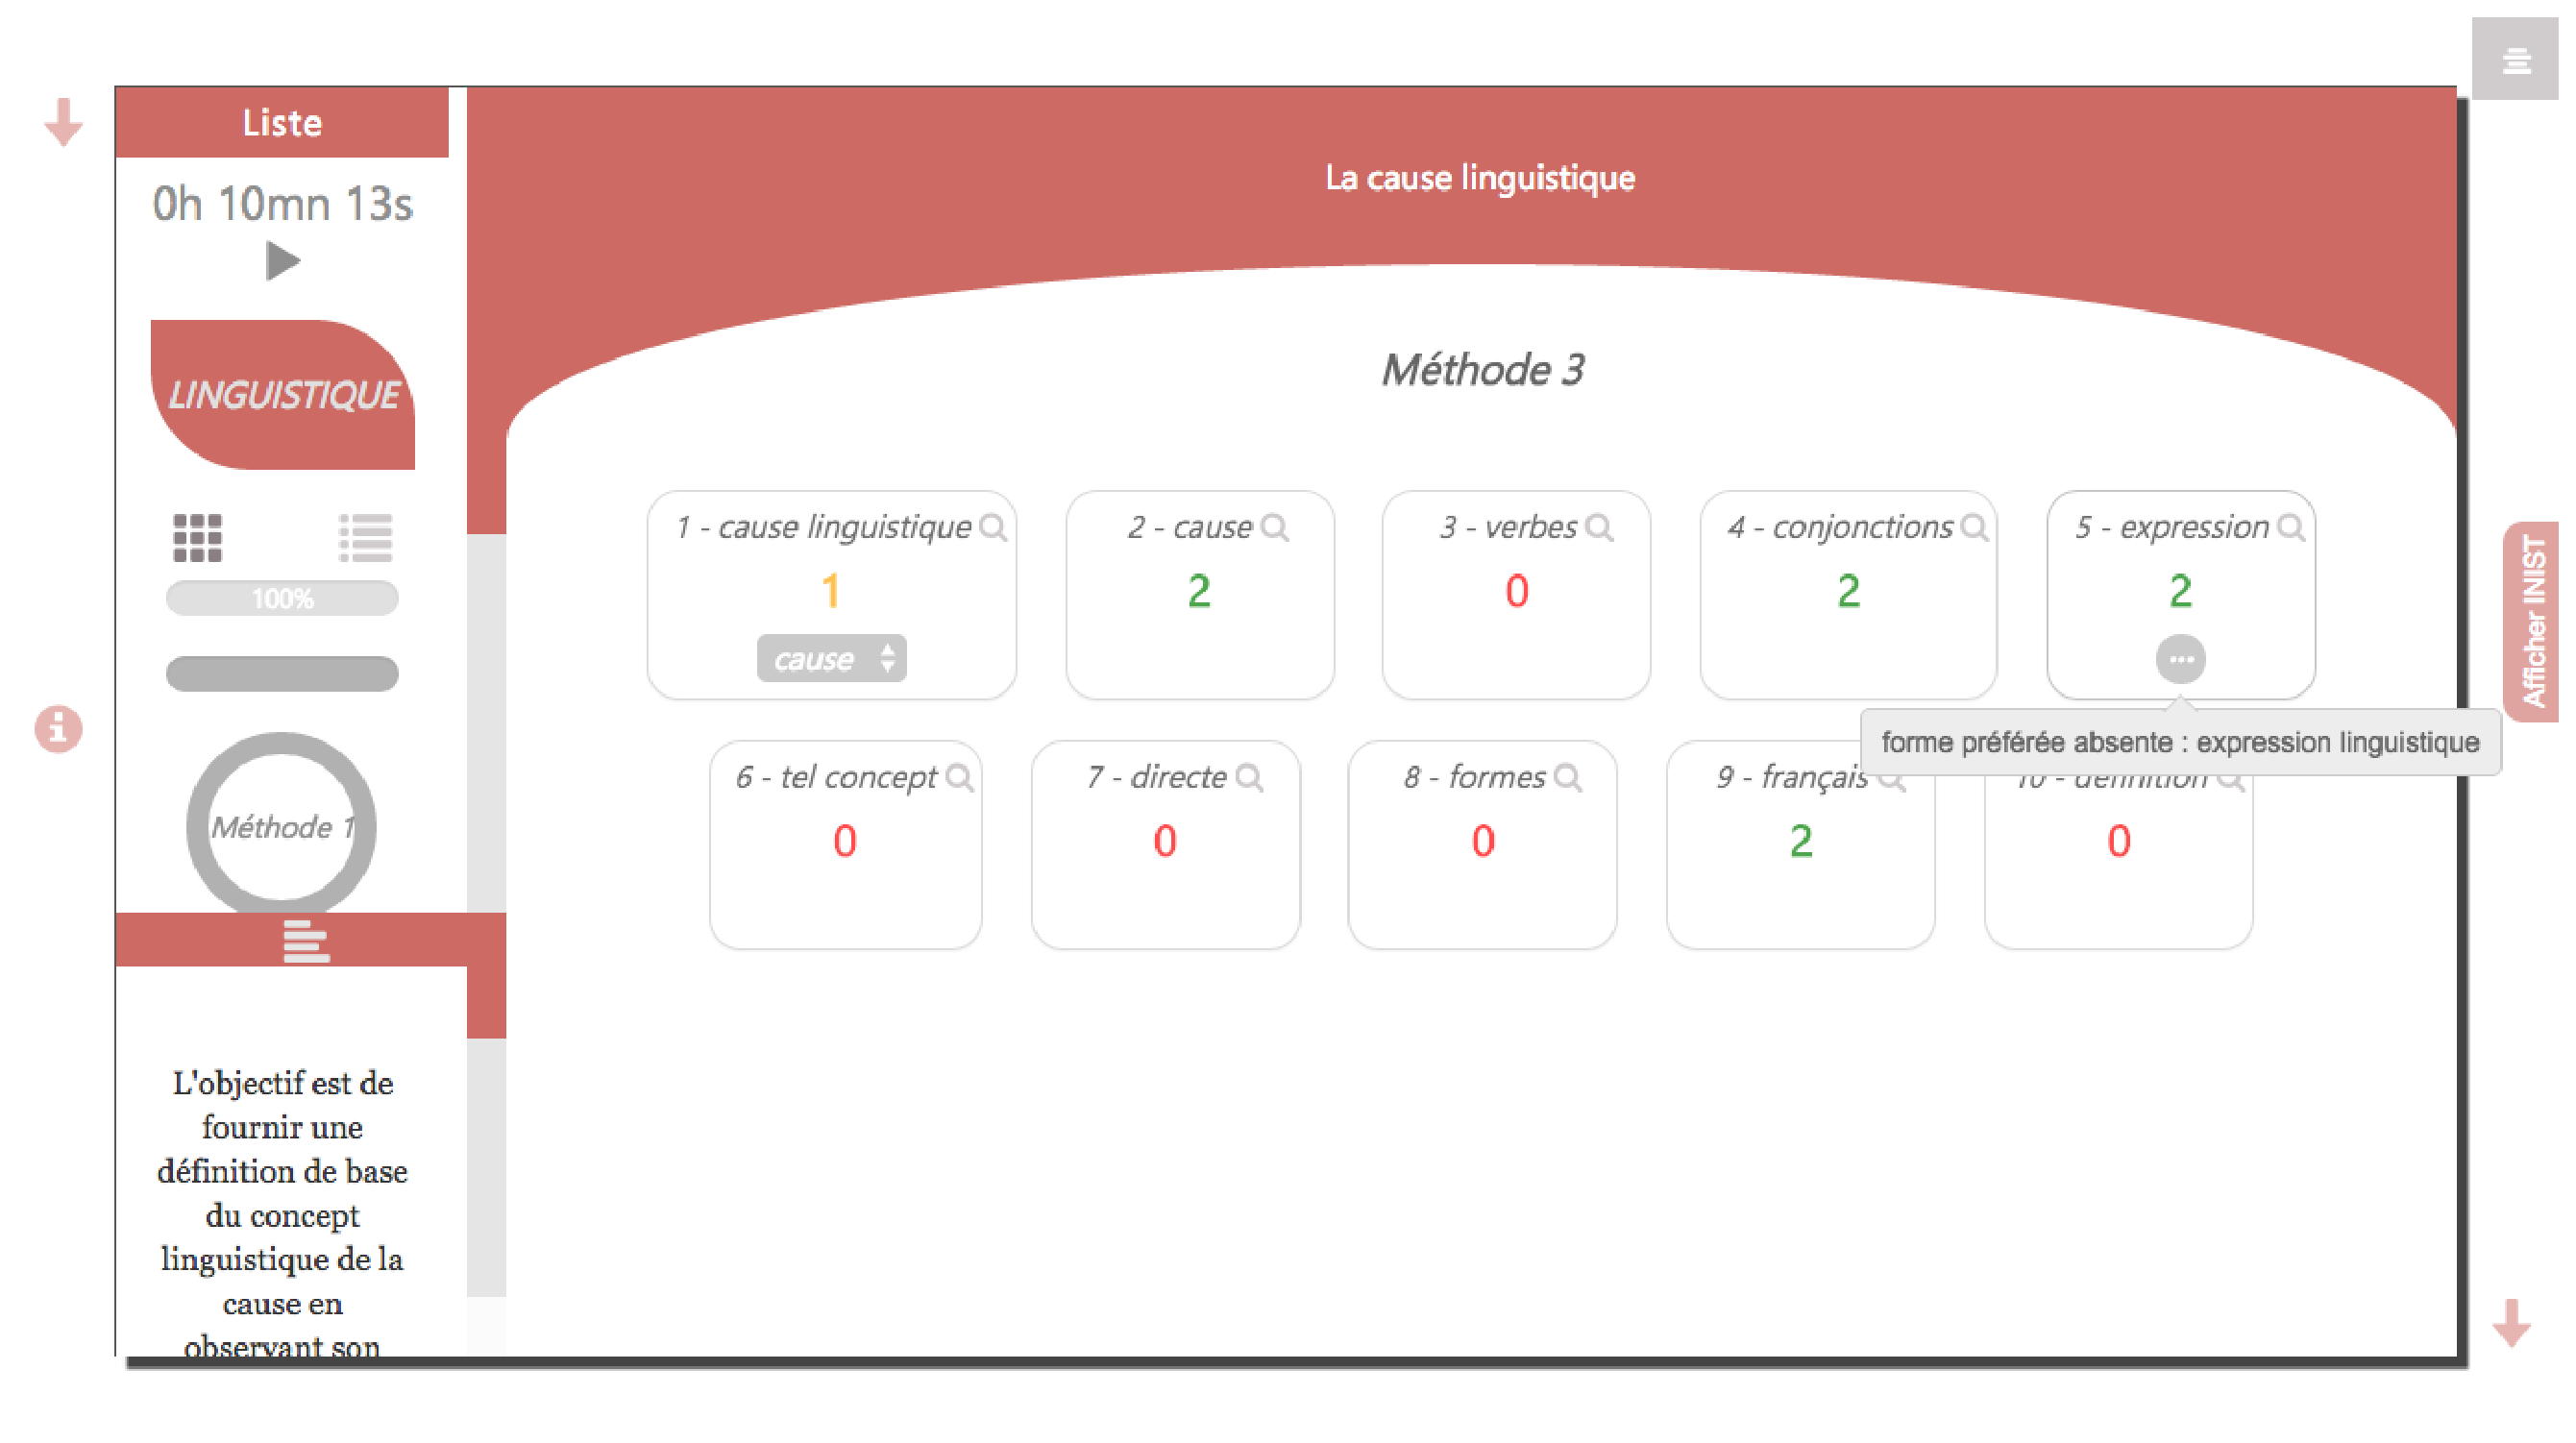
\includegraphics[width=\linewidth]{include/idefix.eps}
          \caption{Interface d'évaluation manuelle\index{evaluation manuelle@Évaluation manuelle} de l'Inist
                   \label{fig:idefix}}
        \end{figure}

      \subsubsection{Évaluation du silence}
      \label{subsubsec:main-automatic_evaluation_of_keyphrase_annotation-methodology-evaluation_protocol-silence}
        Pour évaluer le silence, l'évaluateur doit attribuer à chaque terme-clé\index{terme-cle@Terme-clé}
        de référence\index{reference@Référence} un score\index{score@Score} indiquant le degré d'importance\index{importance@Importance} de l'information
        qu'il véhicule et qui n'est pas capturée par les termes-clés\index{terme-cle@Terme-clé} fournis par
        une méthode\index{methode@Méthode} d'indexation par termes-clés\index{terme-cle@Terme-clé}. Sur une échelle de 0 à 2, ce
        score\index{score@Score} permet d'indiquer s'il n'y pas de perte d'information (0), si
        l'information perdue est capitale (2) ou si elle est secondaire (1).
        Lorsqu'un terme-clé\index{terme-cle@Terme-clé} de référence\index{reference@Référence} obtient un score\index{score@Score} de 0, cela signifie
        soit qu'il fait partie des termes-clés\index{terme-cle@Terme-clé} fournis par la méthode\index{methode@Méthode}
        d'indexation par termes-clés\index{terme-cle@Terme-clé}, soit que l'indexeur juge qu'il ne devrait
        pas être un terme-clé\index{terme-cle@Terme-clé} de référence\index{reference@Référence}, c'est-à-dire une erreur parmi les
        termes-clés\index{terme-cle@Terme-clé} de référence\index{reference@Référence}.

        Une perte d'information est jugée secondaire (score\index{score@Score} de 1) dans deux
        cas de figure~:
        \begin{itemize}
          \item{terme-clé\index{terme-cle@Terme-clé} de référence\index{reference@Référence} secondaire~: le terme-clé\index{terme-cle@Terme-clé} de référence\index{reference@Référence}
                n'apporte pas l'information la plus importante~;}
          \item{terme-clé\index{terme-cle@Terme-clé} de référence\index{reference@Référence} générique~: le terme-clé\index{terme-cle@Terme-clé} de référence\index{reference@Référence}
                n'est pas suffisamment spécifique au contenu du document\index{document@Document}, il a
                un usage classificatoire.}
        \end{itemize}
        Afin de minimiser les pertes d'informations dues à des termes-clés\index{terme-cle@Terme-clé} de
        référence\index{reference@Référence} qui ne sont pas présents dans le document\index{document@Document}, les évaluateurs
        leur attribuent un score\index{score@Score} de 1.

    \subsection{Évaluation manuelle\index{evaluation manuelle@Évaluation manuelle} des méthodes\index{methode@Méthode} proposées}
    \label{subsec:main-domain_specific_keyphrase_annotation-manual_evaluation-analysis}
      Dans cette section, nous analysons l'évaluation manuelle\index{evaluation manuelle@Évaluation manuelle} de TopicRank\index{topicrank@TopicRank},
      TopicCoRank\index{topiccorank@TopicCoRank}, d'une méthode\index{methode@Méthode} de référence\index{reference@Référence} non supervisée, \textsc{Tf-Idf\index{tf-idf@TF-IDF}},
      et d'une méthode\index{methode@Méthode} de référence\index{reference@Référence} supervisée, \textsc{Kea}\footnote{La raison
      pour laquelle les évaluations
      manuelles sont réalisées sur \textsc{Kea} et non pas \textsc{Kea++} est
      temporelle. L'évaluation manuelle\index{evaluation manuelle@Évaluation manuelle} étant coûteuse, nous n'avons pas pu
      la réitérer avec \textsc{Kea++}.}. L'évaluation est
      effectuée par un indexeur professionnel, sur la collection de linguistique
      Termith.

      Dans un premier temps, nous analysons l'évaluation manuelle\index{evaluation manuelle@Évaluation manuelle} de TopicRank\index{topicrank@TopicRank}
      et la comparons à celle de \textsc{Tf-Idf\index{tf-idf@TF-IDF}}, puis, dans un second temps,
      nous analysons l'évaluation manuelle\index{evaluation manuelle@Évaluation manuelle} de TopicCoRank\index{topiccorank@TopicCoRank} et la comparons à
      celle de \textsc{Kea}. Tous les termes-clés\index{terme-cle@Terme-clé} sont obtenus à partir des
      documents\index{document@Document} prétraités, comme nous l'avons présenté dans la
      section~\ref{sec:main-data_description-preprocessing}
      (page~\pageref{sec:main-data_description-preprocessing}). Les candidats
      sont sélectionnés à l'aide du patron grammatical \texttt{/(N|A)+/}.

      \subsubsection{Évaluation de TopicRank\index{topicrank@TopicRank}}
      \label{subsubsec:main-domain_specific_keyphrase_annotation-manual_evaluation-analysis-topicrank}
        Le
        tableau\index{tableau@Tableau}~\ref{tab:main-automatic_evaluation_of_keyphrase_annotation-results-topicrank-pertinence_score_ratio}
        montre les scores\index{score@Score} de pertinence moyens de TopicRank\index{topicrank@TopicRank} et \textsc{Tf-Idf\index{tf-idf@TF-IDF}}. Pour le score\index{score@Score}
        de 1, qui indique qu'un terme-clé\index{terme-cle@Terme-clé} est un forme variante, nous
        distinguons le cas où la variante est redondante\index{redondant@Redondant} du cas où elle ne l'est
        pas. Nous observons que TopicRank\index{topicrank@TopicRank} est meilleur\index{meilleur@Meilleur} que
        \textsc{Tf-Idf\index{tf-idf@TF-IDF}}. TopicRank\index{topicrank@TopicRank} fournit plus de termes-clés\index{terme-cle@Terme-clé} pertinents que
        \textsc{Tf-Idf\index{tf-idf@TF-IDF}}, mais fait aussi plus d'erreurs. Les termes-clés\index{terme-cle@Terme-clé} ayant
        un score\index{score@Score} de 1 donnent un explication intéressante à cette
        contradiction~: \textsc{Tf-Idf\index{tf-idf@TF-IDF}} à une forte tendance à extraire des
        termes-clés\index{terme-cle@Terme-clé} redondants\index{redondant@Redondant}, c'est-à-dire des termes-clés\index{terme-cle@Terme-clé} variantes de
        termes-clés\index{terme-cle@Terme-clé} déjà extraits, alors que TopicRank\index{topicrank@TopicRank} remplit son
        objectif de ne pas extraire de termes-clés\index{terme-cle@Terme-clé} redondants\index{redondant@Redondant}, avec seulement
        0,9~\% de redondance.
        \begin{table}[h!]
          \centering
          \begin{tabular}{l|c|c|c|c}
            \toprule
            \multirow{2}{*}{\textbf{Méthode}} & \multirow{2}{*}{\textbf{0}} & \multicolumn{2}{c|}{\textbf{1}} & \multirow{2}{*}{\textbf{2}}\\
            \cline{3-4}
            & & \multicolumn{1}{p{.175\linewidth}|}{\centering{}redondant} & \multicolumn{1}{p{.175\linewidth}|}{\centering{}non redondant} &\\
            \hline
            \textsc{Tf-Idf} & \textbf{53,8~\%} & 6,8~\% & 4,2~\% & 35,3~\%\\
            TopicRank & 56,3~\% & \textbf{0,9~\%} & \textbf{5,7~\%} & \textbf{37,1~\%}\\
            \bottomrule
          \end{tabular}
          \caption{Taux de termes-clés avec un score de 0, de 1 ou de 2 pour
                   l'évaluation de la pertinence de \textsc{Tf-Idf} et de
                   TopicRank
                   \label{tab:main-automatic_evaluation_of_keyphrase_annotation-results-topicrank-pertinence_score_ratio}}
        \end{table}

        Les résultats\index{resultat@Résultat} présentés dans le
        tableau\index{tableau@Tableau}~\ref{tab:main-automatic_evaluation_of_keyphrase_annotation-results-topicrank-pertinence_score_ratio}
        sont contraires à ceux de l'évaluation automatique, puisque c'est ici
        TopicRank\index{topicrank@TopicRank} qui est meilleur\index{meilleur@Meilleur} que \textsc{Tf-Idf\index{tf-idf@TF-IDF}} sur les documents\index{document@Document} de
        linguistique. Afin de mieux observer la différence entre l'évaluation
        manuelle et l'évaluation automatique, nous calculons la précision (P),
        le rappel (R) et la f1-mesure (F) résultantes de l'évaluation
        manuelle et les comparons aux résultats\index{resultat@Résultat} automatiques que nous avons
        montré dans le tableau\index{tableau@Tableau}~\ref{tab:resultats_inist}
        (page~\pageref{tab:resultats_inist}). Pour calculer ces performances\index{performance@Performance},
        les termes-clés\index{terme-cle@Terme-clé} ayant un score\index{score@Score} de 2 sont considérés corrects, de même
        que ceux ayant un score\index{score@Score} de 1 non redondants\index{redondant@Redondant}. Les résultats\index{resultat@Résultat} de
        l'évaluation manuelle\index{evaluation manuelle@Évaluation manuelle} comparés à ceux de l'évaluation automatique sont
        présentés dans le
        tableau\index{tableau@Tableau}~\ref{tab:main-automatic_evaluation_of_keyphrase_annotation-results-topicrank-prf}.
        
        La difficulté d'évaluer automatiquement la tâche d'indexation par
        termes-clés\index{terme-cle@Terme-clé} se confir\-me. Avec l'évaluation manuelle\index{evaluation manuelle@Évaluation manuelle}, les conclusions ne
        sont pas les mêmes, puisque de manière automatique TopicRank\index{topicrank@TopicRank} est moins
        performant que \textsc{Tf-Idf\index{tf-idf@TF-IDF}} alors qu'il est plus performant selon
        l'évaluation manuelle\index{evaluation manuelle@Évaluation manuelle}. Nous observons aussi un écart conséquent entre
        les performances\index{performance@Performance} évaluées manuellement et celles évaluées
        automatiquement. Le gain d'environ 20 points atteste le pessimisme de
        l'évaluation automatique.
        \begin{table}[h!]
          \centering
          \begin{tabular}{l|c@{~~~~~~}cc|c@{~~~~~~~~}cc}
            \toprule
            \multirow{2}{*}{\textbf{Méthode}} & \multicolumn{3}{c|}{\textbf{Évaluation manuelle}} & \multicolumn{3}{c}{\textbf{Évaluation automatique}}\\
            \cline{2-7}
            & P & R & F & P & R & F\\
            \hline
            \textsc{Tf-Idf} & 39,5 & 29,7 & 33,5 & \textbf{13,0} & \textbf{15,4} & \textbf{13,9}\\
            TopicRank & \textbf{42,8} & \textbf{32,2} & \textbf{36,2} & 11,2 & 13,1 & 11,9\\
            \bottomrule
          \end{tabular}
          \caption[
            Performances de \textsc{Tf-Idf} et de TopicRank en termes de
            précision, de rappel et de f1-mesure
          ]{
            Performances de \textsc{Tf-Idf} et de TopicRank en termes de
            précision (P), de rappel (R) et de f1-mesure (F)
            \label{tab:main-automatic_evaluation_of_keyphrase_annotation-results-topicrank-prf}}
        \end{table}
      
        ~\\Enfin, le
        tableau\index{tableau@Tableau}~\ref{tab:main-automatic_evaluation_of_keyphrase_annotation-results-topicrank-silence_score_ratio}
        montre les scores\index{score@Score} de silence attribués en moyenne par méthode\index{methode@Méthode}. D'après
        la description donnée pour chacun des scores\index{score@Score}, la méthode\index{methode@Méthode} qui capture le
        plus d'information est celle qui maximise le nombre\index{nombre@Nombre} de termes-clés\index{terme-cle@Terme-clé} de
        référence\index{reference@Référence} ayant un score\index{score@Score} de silence 0 et qui minimise ceux ayant un
        score\index{score@Score} de 1 et de 2. Nous observons donc que TopicRank\index{topicrank@TopicRank} couvre mieux le
        contenu principal des documents\index{document@Document} que \textsc{Tf-Idf\index{tf-idf@TF-IDF}}. Parce que TopicRank\index{topicrank@TopicRank}
        groupe les termes-clés\index{terme-cle@Terme-clé} candidats en sujets\index{sujet@Sujet} et n'extrait qu'un seul
        terme-clé\index{terme-cle@Terme-clé} par sujet\index{sujet@Sujet}, il y a moins de redondance parmi les termes-clés\index{terme-cle@Terme-clé}
        qu'il extrait (voir le
        tableau\index{tableau@Tableau}~\ref{tab:main-automatic_evaluation_of_keyphrase_annotation-results-topicrank-pertinence_score_ratio})
        et le nombre\index{nombre@Nombre} de sujets\index{sujet@Sujet} couverts est donc meilleur\index{meilleur@Meilleur}.
        \begin{table}[h!]
          \centering
          \begin{tabular}{l|c|c|c}
            \toprule
            \textbf{Méthode} & \textbf{0} & \textbf{1} & \textbf{2}\\
            \hline
            \textsc{Tf-Idf} & 31,4~\% & 48,5~\% & 20,1~\%\\
            TopicRank & \textbf{35,0~\%} & \textbf{48,3~\%} & \textbf{16,8~\%}\\
            \bottomrule
          \end{tabular}
          \caption{Taux de termes-clés de référence avec un score de 0, de 1 ou
                   de 2 pour l'évaluation du silence de \textsc{Tf-Idf} et de
                   TopicRank
                   \label{tab:main-automatic_evaluation_of_keyphrase_annotation-results-topicrank-silence_score_ratio}}
        \end{table}

      \subsubsection{Évaluation de TopicCoRank\index{topiccorank@TopicCoRank}}
      \label{subsubsec:main-domain_specific_keyphrase_annotation-manual_evaluation-analysis-topiccorank}
        Les résultats\index{resultat@Résultat} que nous montrons dans cette section sont obtenus avec
        seulement 25~\% de l'ensemble\index{ensemble@Ensemble} de test de la collection linguistique
        Termith\footnote{En raison de cette incomplétude de l'évaluation
        manuelle, nous ne comparons pas l'évaluation manuelle\index{evaluation manuelle@Évaluation manuelle} à l'évaluation
        automatique comme nous l'avons fait pour TopicRank\index{topicrank@TopicRank} et \textsc{Tf-Idf\index{tf-idf@TF-IDF}}.}.
        Les différentes revues qui composent la collection sont
        réparties de manière homogène dans ces 25~\%.

        Le
        tableau\index{tableau@Tableau}~\ref{tab:main-domain_specific_keyphrase_annotation-manual_evaluation-analysis-topiccorank-pertinence_score_ratio}
        montre les scores\index{score@Score} de pertinence moyens de TopicCoRank\index{topiccorank@TopicCoRank} et \textsc{Kea}.
        Nous observons que TopicCoRank\index{topiccorank@TopicCoRank} est meilleur\index{meilleur@Meilleur} que
        \textsc{Kea}. TopicCoRank\index{topiccorank@TopicCoRank} fournit plus de termes-clés\index{terme-cle@Terme-clé} pertinents que
        \textsc{Kea}, mais fait aussi plus d'erreurs. À l'instar de TopicRank\index{topicrank@TopicRank},
        TopicCoRank\index{topiccorank@TopicCoRank} est moins redondant\index{redondant@Redondant} que la méthode\index{methode@Méthode} de référence\index{reference@Référence}. Il est tout
        de même plus redondant\index{redondant@Redondant} que TopicRank\index{topicrank@TopicRank}. Cela est du au fait qu'il peut assigner un terme-clé\index{terme-cle@Terme-clé} et
        extraire une variante pouvant être jugée importante, car plus
        spécifique, ou redondante\index{redondant@Redondant}.
        \begin{table}[h!]
          \centering
          \begin{tabular}{l|c|c|c|c}
            \toprule
            \multirow{2}{*}{\textbf{Méthode}} & \multirow{2}{*}{\textbf{0}} & \multicolumn{2}{c|}{\textbf{1}} & \multirow{2}{*}{\textbf{2}}\\
            \cline{3-4}
            & & \multicolumn{1}{p{.175\linewidth}|}{\centering{}redondant} & \multicolumn{1}{p{.175\linewidth}|}{\centering{}non redondant} &\\
            \hline
            \textsc{Kea} & \textbf{45,2~\%} & 10,2~\% & \textbf{8,0~\%} & 36,6~\%\\
            TopicCoRank & 49,8~\% & \textbf{4,4~\%} & 6,2~\% & \textbf{39,6~\%}\\
            \bottomrule
          \end{tabular}
          \caption{Taux de termes-clés avec un score de 0, de 1 ou de 2 pour
                   l'évaluation de la pertinence de \textsc{Kea} et de
                   TopicCoRank
                   \label{tab:main-domain_specific_keyphrase_annotation-manual_evaluation-analysis-topiccorank-pertinence_score_ratio}}
        \end{table}

        Comparé à TopicRank\index{topicrank@TopicRank}, TopicCoRank\index{topiccorank@TopicCoRank} est effectivement plus performant. Il
        trouve plus de termes-clés\index{terme-cle@Terme-clé} corrects et fait moins d'erreurs. Cependant,
        comme nous
        l'avons dit ci-dessus, il est plus redondant\index{redondant@Redondant}. Comparée à
        \textsc{Tf-Idf\index{tf-idf@TF-IDF}} et \textsc{Kea}, cette redondance est tout de même plus
        faible.

%        \TODO{\dots}
%        \begin{table}[h!]
%          \centering
%          \begin{tabular}{l|c@{~~~~~~}cc|c@{~~~~~~~~}cc}
%            \toprule
%            \multirow{2}{*}{\textbf{Méthode\index{methode@Méthode}}} & \multicolumn{3}{c|}{\textbf{Évaluation manuelle\index{evaluation manuelle@Évaluation manuelle}}} & \multicolumn{3}{c}{\textbf{Évaluation automatique}}\\
%            \cline{2-7}
%            & P & R & F & P & R & F\\
%            \hline
%            \textsc{Kea} & 44,6 & 32,5 & 37,1 & 13,8 & 16,3 & 14,7\\
%            TopicCoRank\index{topiccorank@TopicCoRank} & \textbf{45,8} & \textbf{34.1} & \textbf{39.6} & \textbf{19,0} & \textbf{22,0} & \textbf{20,1}\\
%            \bottomrule
%          \end{tabular}
%          \caption[
%            Performances\index{performance@Performance} de \textsc{Kea} et de TopicCoRank\index{topiccorank@TopicCoRank} en termes de
%            précision, de rappel et de f-mesure
%          ]{
%            Performances\index{performance@Performance} de \textsc{Kea} et de TopicCoRank\index{topiccorank@TopicCoRank} en termes de
%            précision (P), de rappel (R) et de f-mesure (F)
%            \label{tab:main-domain_specific_keyphrase_annotation-manual_evaluation-analysis-topiccorank-prf}}
%        \end{table}
      
        ~\\Enfin, le
        tableau\index{tableau@Tableau}~\ref{tab:main-domain_specific_keyphrase_annotation-manual_evaluation-analysis-topiccorank-silence_score_ratio}
        montre les scores\index{score@Score} de silence attribués en moyenne par méthode\index{methode@Méthode}. Les
        conclusions qu'ils induisent ne sont pas en faveur de
        TopicCoRank\index{topiccorank@TopicCoRank}. En effet, même s'il ne capture pas autant de termes-clés\index{terme-cle@Terme-clé}
        que TopicCoRank\index{topiccorank@TopicCoRank}, \textsc{Kea} capture ceux qui sont sémantiquement les
        plus indispensables. Bien que les deux méthodes\index{methode@Méthode} sont supervisées,
        \textsc{Kea} est la seule des deux à apprendre à détecter les
        termes-clés\index{terme-cle@Terme-clé} à partir des traits des termes-clés\index{terme-cle@Terme-clé} du domaine\index{domaine@Domaine}. Si
        l'ordonnancement conjoint\index{conjoint@Conjoint} à base de graphe\index{graphe@Graphe} est plus efficace pour
        identifier les termes-clés\index{terme-cle@Terme-clé}, l'apprentissage permet une meilleure\index{meilleur@Meilleur}
        précision quant à l'identification de ceux les plus indispensables.
        \begin{table}[h!]
          \centering
          \begin{tabular}{l|c|c|c}
            \toprule
            \textbf{Méthode} & \textbf{0} & \textbf{1} & \textbf{2}\\
            \hline
            \textsc{Kea} & \textbf{37,3~\%} & 46,0~\% & \textbf{16,7}~\%\\
            TopicCoRank & 35,9~\% & \textbf{45,3~\%} & 18,8~\%\\
            \bottomrule
          \end{tabular}
          \caption{Taux de termes-clés de référence avec un score de 0, de 1 ou
                   de 2 pour l'évaluation du silence de \textsc{Kea} et de
                   TopicCoRank
                   \label{tab:main-domain_specific_keyphrase_annotation-manual_evaluation-analysis-topiccorank-silence_score_ratio}}
        \end{table}

    \subsection{Bilan}
    \label{subsec:main-domain_specific_keyphrase_annotation-manual_evaluation-conclusion}
      Nous avons réalisé une campagne d'évaluation manuelle\index{evaluation manuelle@Évaluation manuelle} de nos travaux en
      domaine\index{domaine@Domaine} de spécialité\index{specialite@Spécialité}, avec la collection de linguistique Termith. Pour
      cette campagne, nous avons proposé un protocole d'évaluation et des
      métriques permettant de capturer deux aspects de l'indexation par
      termes-clés\index{terme-cle@Terme-clé}~: la pertinence des termes-clés\index{terme-cle@Terme-clé} extraits/assignés et leur
      silence, c'est-à-dire la quantité d'information importante qu'ils ne
      capturent pas. Contrairement au premier aspect, qui est similaire à ce
      qu'évalue un système automatique, le dernier aspect permet d'évaluer les
      termes-clés\index{terme-cle@Terme-clé} d'un point de vu sémantique, jamais considéré auparavant.

      Les résultats\index{resultat@Résultat} montrent que, contrairement à ce que montrait l'évaluation
      automatique, TopicRank\index{topicrank@TopicRank} effectue une indexation par termes-clés\index{terme-cle@Terme-clé} de
      meilleure\index{meilleur@Meilleur} qualité que celle de \textsc{Tf-Idf\index{tf-idf@TF-IDF}}. TopicRank\index{topicrank@TopicRank} extrait peu de
      termes-clés\index{terme-cle@Terme-clé} redondants\index{redondant@Redondant} et couvre mieux le document\index{document@Document}, en partie grâce à son
      groupement des termes-clés\index{terme-cle@Terme-clé} candidats en sujets\index{sujet@Sujet}. Entre TopicCoRank\index{topiccorank@TopicCoRank},
      TopicRank\index{topicrank@TopicRank}, \textsc{Tf-Idf\index{tf-idf@TF-IDF}} et \textsc{Kea}, c'est TopicCoRank\index{topiccorank@TopicCoRank} qui trouve
      le plus de termes-clés\index{terme-cle@Terme-clé} corrects. L'évaluation du silence montre tout de
      même que c'est \textsc{Kea} qui identifie ceux jugés les plus
      indispensables par les indexeurs professionnels. Les deux aspects
      (pertinence et silence) de l'évaluation manuelle\index{evaluation manuelle@Évaluation manuelle} et leurs conclusions
      paradoxales soulèvent une nouvelle perspective pour l'évaluation
      automatique. En effet, il serait intéressant d'ordonner par importance\index{importance@Importance} les
      termes-clés\index{terme-cle@Terme-clé} de référence\index{reference@Référence} et d'en tenir compte pour identifier les méthodes\index{methode@Méthode}
      qui capturent les termes-clés\index{terme-cle@Terme-clé} les plus indispensables.

  %-----------------------------------------------------------------------------

  \section{Conclusion}
  \label{sec:main-domain_specific_keyphrase_annotation-conclusion}
    Nous nous sommes intéressé à l'indexation automatique\index{indexation automatique@Indexation automatique} par termes-clés\index{terme-cle@Terme-clé} en
    domaines\index{domaine@Domaine} de spécialité\index{specialite@Spécialité}. Nous avons tout d'abord présenté l'indexation
    manuelle réalisée par des indexeurs professionnels dans ce contexte, nous
    avons ensuite proposé une nouvelle méthode\index{methode@Méthode} automatique se rapprochant le
    plus possible de cette indexation, puis nous avons présenté les premiers
    résultats\index{resultat@Résultat} d'une campagne d'évaluation manuelle\index{evaluation manuelle@Évaluation manuelle} que nous avons réalisé avec
    des indexeurs professionnels.

    Contrairement aux méthodes\index{methode@Méthode} d'indexation automatique\index{indexation automatique@Indexation automatique}, l'indexation manuelle
    n'est pas divisée entre extraction et assignement. L'indexation manuelle en
    domaines\index{domaine@Domaine} de spécialité\index{specialite@Spécialité} préfère l'assignement, car cela permet une
    indexation homogène des documents\index{document@Document} d'un même domaine\index{domaine@Domaine} et une conformité
    vis-à-vis du vocabulaire\index{vocabulaire@Vocabulaire} spécialisé du domaine\index{domaine@Domaine}. Elle a aussi besoin de
    l'extraction, afin de fournir des termes-clés\index{terme-cle@Terme-clé} très spécifiques au document\index{document@Document},
    ainsi que pour y identifier d'éventuels nouveaux concepts.

    Pour remédier à la fracture entre extraction et assignement en indexation
    automatique par termes-clés\index{terme-cle@Terme-clé}, nous proposons TopicCoRank\index{topiccorank@TopicCoRank}. Conçu sur la base
    de TopicRank\index{topicrank@TopicRank}, TopicCoRank\index{topiccorank@TopicCoRank} utilise les données d'entraînement pour
    représenter le domaine\index{domaine@Domaine} avec un graphe\index{graphe@Graphe} unifié à celui des sujets\index{sujet@Sujet}. Cette
    unification permet d'améliorer l'ordonnancement des sujets\index{sujet@Sujet}, en tenant compte
    de leurs relations avec le domaine\index{domaine@Domaine}, et d'assigner des termes-clés\index{terme-cle@Terme-clé}, en
    puisant dans le domaine\index{domaine@Domaine}. À notre connaissance, TopicCoRank\index{topiccorank@TopicCoRank} est la seule
    méthode\index{methode@Méthode} qui réalise conjointement extraction et assignement.

    Pour valider les deux méthodes\index{methode@Méthode} TopicRank\index{topicrank@TopicRank} et TopicCoRank\index{topiccorank@TopicCoRank}, nous avons réalisé
    une campagne d'évaluation manuelle\index{evaluation manuelle@Évaluation manuelle} en domaine\index{domaine@Domaine} de spécialité\index{specialite@Spécialité}. Le protocole
    d'évaluation que nous avons proposé permet d'évaluer chaque méthode\index{methode@Méthode} selon le
    degré de pertinence des termes-clés\index{terme-cle@Terme-clé} qu'elle propose et selon le degré
    d'information qui lui échappe. Les résultats\index{resultat@Résultat} de l'évaluation manuelle\index{evaluation manuelle@Évaluation manuelle} de
    TopicRank\index{topicrank@TopicRank} son plus encourageant que ceux de l'évaluation automatique. Ils
    montrent que TopicRank\index{topicrank@TopicRank} est en réalité plus performant que \textsc{Tf-Idf\index{tf-idf@TF-IDF}},
    en partie parce qu'il couvre mieux les sujets\index{sujet@Sujet} du document\index{document@Document} grâce à son
    groupement en sujets\index{sujet@Sujet} des termes-clés\index{terme-cle@Terme-clé} candidats.
    Ils montrent aussi que TopicCoRank\index{topiccorank@TopicCoRank} est la méthode\index{methode@Méthode} la plus performante
    comparée à TopicRank\index{topicrank@TopicRank}, \textsc{Tf-Idf\index{tf-idf@TF-IDF}} et \textsc{Kea}. Cependant, c'est
    \textsc{Kea} qui trouve les termes-clés\index{terme-cle@Terme-clé} les plus indispensables.
    Au delà de cela, cette
    campagne a montré les limites de l'évaluation automatique, qui suit un
    paradigme trop strict pour la tâche d'indexation par termes-clés\index{terme-cle@Terme-clé}. Parce que
    l'évaluation manuelle\index{evaluation manuelle@Évaluation manuelle} est trop coûteuse pour être systématiquement mise en
    \oe{}uvre, il est donc important de s'intéresser de plus près aux méthodes\index{methode@Méthode}
    d'évaluation automatique. Les ressources de notre campagne, annotées étape
    par étape, seront donc
    rendues disponibles gratuitement à toute la communauté scientifique. Cette
    disponibilité permettra d'évaluer de nouvelles méthodes\index{methode@Méthode} d'évaluation, en
    vérifiant leur corrélation avec l'évaluation manuelle\index{evaluation manuelle@Évaluation manuelle} des indexeurs
    professionnels.

